\chapter{DESENVOLVIMENTO DO PROJETO}
\label{geral-requisitos-gerenciamento}

No desenvolvimento de qualquer projeto, desde os mais simples até os mais complexos, uma fase crucial é a sua concepção e planejamento. Neste capítulo, exploraremos os diversos aspectos envolvidos nesse processo inicial, que nos guiarão durante o desenvolvimento do projeto. Desde a definição dos requisitos e escopo do projeto, passando pela elaboração de casos de uso e arquitetura, até a consideração da infraestrutura necessária para sua implementação, cada etapa desempenha um papel fundamental na construção do produto final. Além disso, discutiremos a importância da manutenibilidade do sistema, sua viabilidade financeira e as diferentes fases de entrega, visando garantir não apenas a entrega de um produto funcional, mas também sua sustentabilidade e sucesso a longo prazo.

\section{Elicitação de Requisitos}
Neste capítulo, vamos explorar o processo de elicitação de requisitos, fundamental para o desenvolvimento de \textit{software}.

\subsection{Requisitos funcionais}

Requisitos funcionais são especificações que descrevem as funções e operações que um sistema ou \textit{software} deve ser capaz de realizar. Eles definem as funcionalidades específicas que o sistema deve fornecer, incluindo entradas, saídas e comportamentos esperados em diferentes cenários de uso. Para a elaboração do projeto, foram definidos oito requisitos funcionais.

\begin{itemize}
    \item \textbf{Funcionalidades das Perguntas do Teste Vocacional:}
    \begin{itemize}
        \item \textbf{RF1} - Manter perguntas do teste vocacional (incluir, alterar, excluir, consultar).
    \end{itemize}

    \item \textbf{Funcionalidades das respostas do Teste Vocacional:}
    \begin{itemize}
        \item \textbf{RF2} - Permitir ao estudante responder o teste.
        \item \textbf{RF3} - Manter respostas do teste vocacional (incluir, consultar).
    \end{itemize}

    \item \textbf{Funcionalidades das Instituições Públicas:}
    \begin{itemize}
        \item \textbf{RF4 }- Manter informações pertinentes sobre os cursos (incluir, alterar, excluir, consultar).
        \item \textbf{RF5} - Disponibilizar informações dos cursos e \ac{ies} cadastradas, permitindo filtragem.
    \end{itemize}

    \item \textbf{Funcionalidades dos Usuários (Administradores e Estudantes):}
    \begin{itemize}
        \item \textbf{RF6} - Manter cadastro dos estudantes (incluir, alterar, excluir, consultar).
        \item \textbf{RF7} - Manter cadastro dos administradores (incluir, alterar, excluir, consultar).
    \end{itemize}

    \item \textbf{Apresentar Resultado de Indicação do Curso:}
    \begin{itemize}
        \item \textbf{RF8} - Apresentar recomendação personalizada de cursos para o estudante após a conclusão do teste vocacional.
    \end{itemize}
    
\end{itemize}

    
\subsection{Requisitos não funcionais}

Requisitos não funcionais referem-se a critérios que não estão diretamente relacionados às funcionalidades específicas do sistema, mas sim a atributos de qualidade, restrições ou características gerais que o sistema deve possuir. Isso inclui aspectos como desempenho, segurança, usabilidade, escalabilidade, confiabilidade e compatibilidade. Esses requisitos definem os padrões de qualidade e comportamento que o sistema deve atender, sem especificar diretamente as funções que ele deve realizar. Para a elaboração do projeto, foram definidos sete requisitos não funcionais

\begin{itemize}
    \item \textbf{Logs:}
    \begin{itemize}
        \item \textbf{RNF1} - Criação de testes e logs do sistema para reconhecimento e tratativa de erros
    \end{itemize}

    \item \textbf{Usabilidade:}
    \begin{itemize}
        \item \textbf{RNF2} - Interface amigável, fácil e intuitiva para todos os tipos de usuários.
    \end{itemize}

    \item \textbf{Desempenho:}
    \begin{itemize}
        \item \textbf{RNF3} - Respostas rápidas às solicitações do usuário, com tempo de carregamento eficiente para as funcionalidades do sistema.
    \end{itemize}

    \item \textbf{Segurança:}
    \begin{itemize}
        \item \textbf{RNF4} - Proteção de dados sensíveis dos usuários, incluindo autenticação e autorização para acessar determinadas funcionalidades.
        \item \textbf{RNF5} - Os dados dos usuários devem ser coletados, armazenados e processados de acordo com a legislação local sobre proteção de dados.
    \end{itemize}

    \item \textbf{Escalabilidade:}
    \begin{itemize}
        \item \textbf{RNF6} - O sistema deve ser capaz de lidar com um aumento no número de usuários e dados sem degradar a performance.
    \end{itemize}

    \item \textbf{Compatibilidade:}
    \begin{itemize}
        \item \textbf{RNF7} - O sistema deve possuir suporte a diferentes navegadores (Chrome, Firefox e Opera GX) e dispositivos (responsividade).
    \end{itemize}

\end{itemize}



\subsection{Regras de negócio}

Dentro de um \textit{software}, as regras de negócio referem-se às diretrizes lógicas que governam o comportamento e as operações do sistema em relação aos processos de negócio da organização. Elas definem as condições, restrições e comportamentos que o \textit{software} deve seguir para garantir que as operações empresariais sejam realizadas de acordo com as políticas e procedimentos estabelecidos.

As regras de negócio definidas para a aplicação Vocco são:
\begin{itemize}
\item {As informações das universidades devem ser atualizadas semestralmente para refletir quaisquer mudanças nas políticas de admissão e nos cursos oferecidos.}
\item {Será permitida a criação de contas para estudantes maiores de 14 anos.}
\item {Só serão permitidos cadastros e recomendações de \ac{ies} públicas. 
}

\end{itemize}


\section{Escopo do projeto}
A definição do escopo do projeto foi embasada na utilização de casos de uso. Essa decisão foi tomada devido à necessidade de uma abordagem estruturada e detalhada para descrever as interações entre os usuários e o sistema. 

Os casos de uso possibilitam uma especificação clara dos requisitos funcionais, identificando de forma precisa as principais funcionalidades do sistema e os comportamentos esperados. 

Portanto, a escolha de utilizar apenas casos de uso foi considerada apropriada para garantir a compreensão precisa do escopo do projeto e assegurar o sucesso da implementação.
\subsection{Casos de Uso}
A seguir, apresenta-se o caso de uso desenvolvido para a plataforma Vocco, apresentado na Figura \ref{casodeuso}, acompanhado de suas descrições. 


        
\begin{figure}[ht]
    \centering
    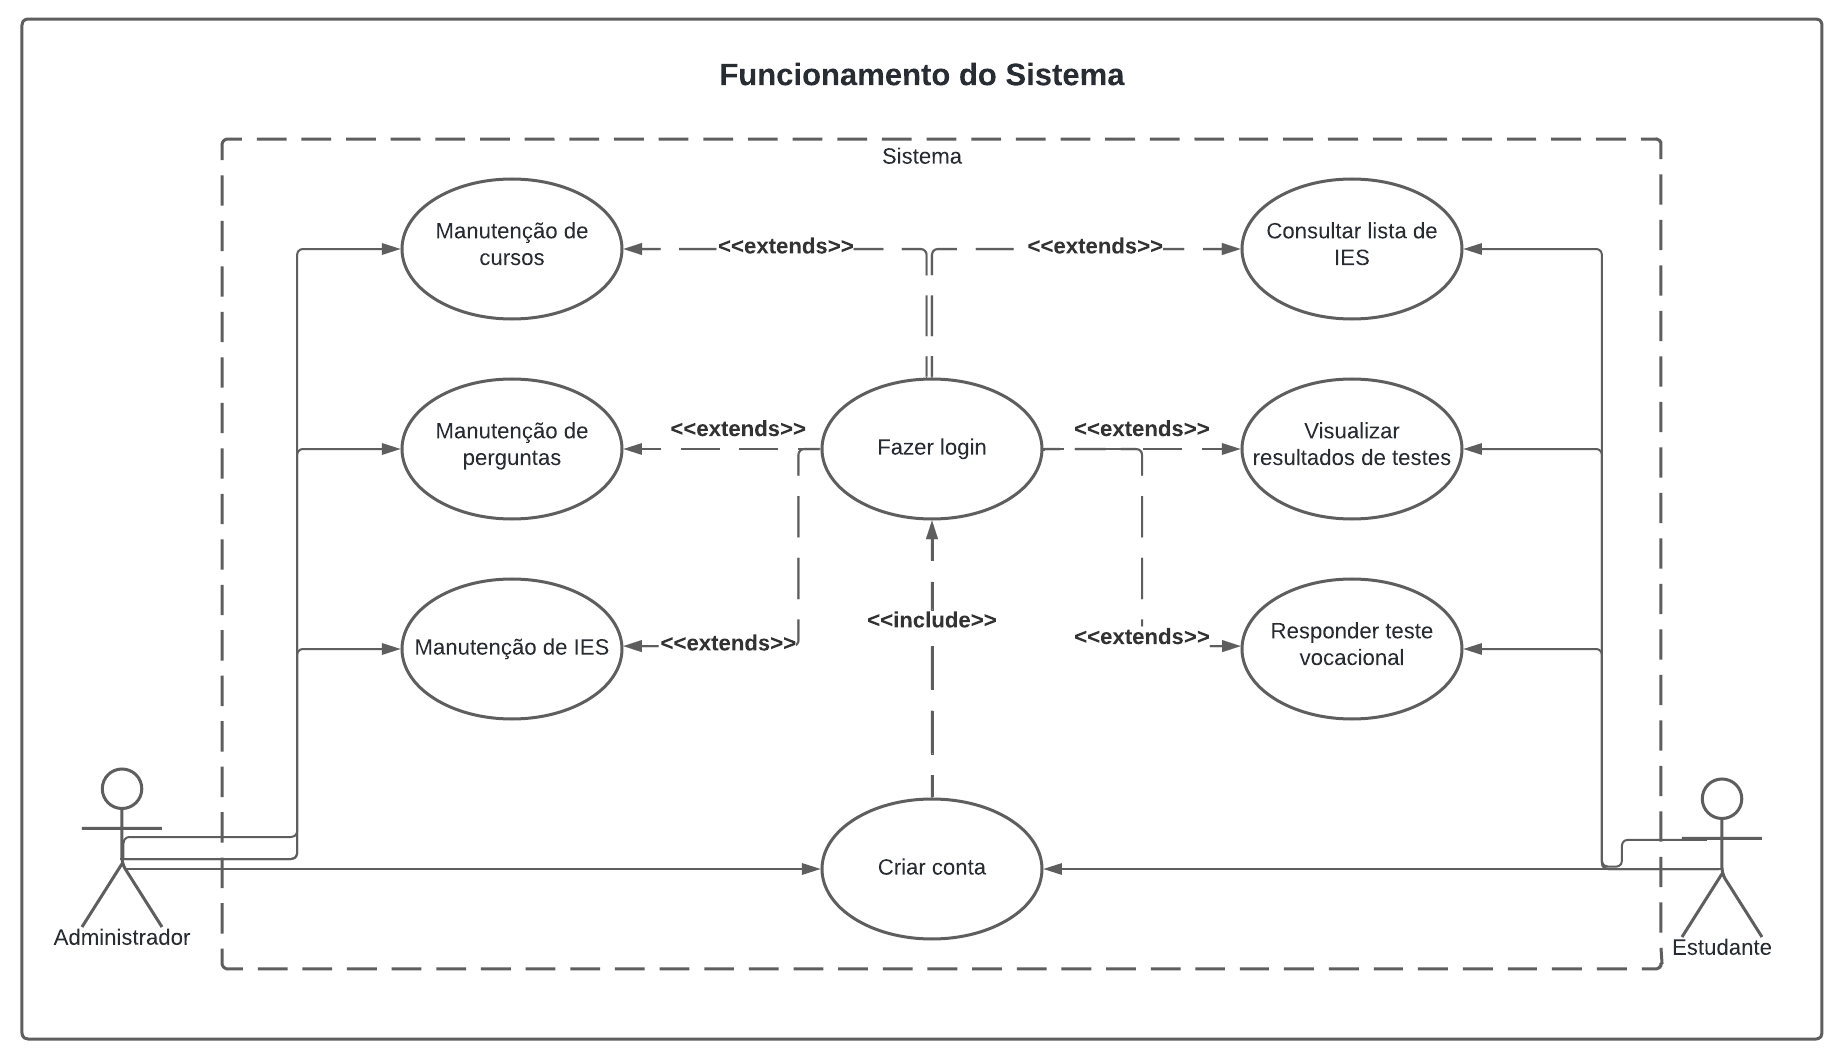
\includegraphics[scale=0.6]{images/caso-de-uso-funcionamento-sistema.png}
    \caption{Caso de Uso: Funcionamento do Sistema}
    \label{casodeuso}
\end{figure}  


\begin{table}[h!]
\centering
\caption{Fluxo de Cadastro de Usuário (Administrador)}
\begin{tabular}{|m{4cm}|m{11cm}|}
\hline
\textbf{Caso de Uso}   & \textbf{Cadastro de Usuário - Administrador} \\
\hline
Ator Principal & Administrador\\
\hline
Interessados e Interesses & O administrador deseja criar e gerenciar sua conta para acessar as funcionalidades de manutenção das perguntas do teste vocacional. \\
\hline
Pré-Condições & O administrador possui permissão para ter um cadastro na plataforma. \\
\hline
Fluxo Básico & 

1. O administrador acessa a página de cadastro.
2. O sistema solicita dados pessoais.
3. O administrador insere os dados.
4. O sistema valida os dados.
5. O sistema verifica se o e-mail é único.
6. O sistema salva os dados.
7. O administrador recebe confirmação de sucesso.\\
\hline
Fluxos Alternativos & 

1. E-mail já em uso: mensagem de erro.
2. E-mail inválido: mensagem de erro.
3. CPF inválido: mensagem de erro.
4. Campos obrigatórios não preenchidos: mensagem de erro.
\\
\hline
Fluxo de Exceção & Falha técnica: mensagem de erro, caso de uso encerrado. \\
\hline
Pós-Condições & Cadastro realizado com sucesso e administrador pode acessar a plataforma. \\
\hline
\end{tabular}
\label{table:casos-de-uso}
\\[1ex]
\footnotesize \textbf{Fonte}: Elaborado pelo autor.
\end{table}



\begin{table}[h!]
\centering
\caption{Fluxo de Cadastro de Instituição Pública}
\begin{tabular}{|m{4cm}|m{11cm}|}
\hline
\textbf{Caso de Uso}   & \textbf{Cadastro de Instituição Pública} \\
\hline
Ator Principal & Administrador\\
\hline
Interessados e Interesses & O administrador deseja cadastrar uma instituição pública na plataforma para disponibilizar informações sobre seus cursos, formas de ingresso e políticas públicas de acesso e permanência. \\
\hline
Pré-Condições & 

1. O administrador possui cadastro na plataforma.
2. A instituição possui as informações necessárias para cadastro.
\\
\hline
Fluxo Básico & 

1. O administrador acessa a funcionalidade de cadastro de instituição.
2. O sistema solicita os dados da instituição.
3. O administrador preenche os dados.
4. O sistema valida os dados.
5. O sistema valida e verifica a unicidade dos dados.
6. O sistema salva os dados.
7. O administrador recebe confirmação de sucesso.
\\
\hline
Fluxos Alternativos & 

1. Nome da instituição já em uso: mensagem de erro.
2. Site inválido: mensagem de erro.
3. Nota do MEC inválida: mensagem de erro.
4. Endereço incompleto: mensagem de erro.
\\
\hline
Fluxo de Exceção & Falha técnica: mensagem de erro, caso de uso encerrado. \\
\hline
Pós-Condições & Instituição pública cadastrada com sucesso na plataforma. \\
\hline
\end{tabular}
\label{table:casos-de-uso}
\\[1ex]
\footnotesize \textbf{Fonte}: Elaborado pelo autor.
\end{table}

\begin{table}[h!]
\centering
\caption{Fluxo de Cadastro de Usuário (Estudante)}
\begin{tabular}{|m{4cm}|m{11cm}|}
\hline
\textbf{Caso de Uso}   & \textbf{Cadastro de Usuário - Estudante} \\
\hline
Ator Principal & Estudante\\
\hline
Interessados e Interesses & O estudante deseja se cadastrar na plataforma para ter acesso ao teste vocacional personalizado e às informações sobre as universidades públicas. \\
\hline
Pré-Condições & O estudante possui mais de 14 anos de idade. \\
\hline
Fluxo Básico & 

1. O estudante acessa a página de cadastro.
2. O sistema solicita dados pessoais.
3. O estudante insere os dados.
4. O sistema valida os dados.
5. O sistema cria a conta e salva os dados.
6. O estudante recebe confirmação de sucesso.
\\
\hline
Fluxos Alternativos & 

1. E-mail inválido: mensagem de erro.
2. Campos obrigatórios não preenchidos: mensagem de erro.
4. Campos obrigatórios não preenchidos: mensagem de erro.
\\
\hline
Fluxo de Exceção & Falha técnica: mensagem de erro, caso de uso encerrado. \\
\hline
Pós-Condições & Cadastro realizado com sucesso e estudante pode acessar a plataforma. \\
\hline
\end{tabular}
\label{table:casos-de-uso}
\\[1ex]
\footnotesize \textbf{Fonte}: Elaborado pelo autor.
\end{table}

\begin{table}[h!]
\centering
\caption{Fluxo de Manter Perguntas do Teste Vocacional}
\begin{tabular}{|m{4cm}|m{11cm}|}
\hline
\textbf{Caso de Uso}   & \textbf{Manter Perguntas do Teste Vocacional} \\
\hline
Ator Principal & Administrador\\
\hline
Interessados e Interesses & O administrador deseja gerenciar as perguntas do teste vocacional para garantir a qualidade e relevância do teste para os estudantes. \\
\hline
Pré-Condições & 

1. O administrador possui acesso ao sistema.
2. Deve haver ao menos uma pergunta cadastrada para alterar/excluir. \\
\hline
Fluxo Básico & 

1. O administrador acessa a funcionalidade de manutenção de perguntas.
2. O sistema exibe a lista de perguntas.
3. O administrador escolhe incluir, alterar, excluir ou consultar uma pergunta.
4. O sistema executa a ação e atualiza a lista.
\\
\hline
Fluxos Alternativos & 

1. Pergunta com texto vazio: mensagem de erro.
2. Pergunta inexistente: mensagem de erro na alteração/exclusão.
\\
\hline
Fluxo de Exceção & Falha técnica: mensagem de erro, caso de uso encerrado. \\
\hline
Pós-Condições & Pergunta incluída, alterada, excluída ou consultada com sucesso, mantendo a qualidade do teste.\\
\hline
\end{tabular}
\label{table:casos-de-uso}
\\[1ex]
\footnotesize \textbf{Fonte}: Elaborado pelo autor.
\end{table}

\begin{table}[h!]
\centering
\caption{Fluxo de Manter Informações sobre Cursos}
\begin{tabular}{|m{4cm}|m{11cm}|}
\hline
\textbf{Caso de Uso}   & \textbf{Manter Informações sobre Cursos} \\
\hline
Ator Principal & Administrador\\
\hline
Interessados e Interesses & O administrador deseja manter informações atualizadas sobre os cursos oferecidos pela instituição pública na plataforma. \\
\hline
Pré-Condições & 

1. O administrador possui acesso à plataforma.
2. A instituição já está cadastrada. \\
\hline
Fluxo Básico & 
1. O administrador acessa a funcionalidade de manutenção de cursos.
2. O sistema apresenta a lista de cursos.
3. O administrador escolhe incluir, alterar, excluir ou consultar um curso.
4. O sistema executa a ação e atualiza a lista.
\\
\hline
Fluxos Alternativos & 

1. Informações incompletas/ inválidas: mensagem de erro na inclusão.
2. Curso inexistente: mensagem de erro na alteração/exclusão.
\\
\hline
Fluxo de Exceção & Falha técnica: mensagem de erro, caso de uso encerrado. \\
\hline
Pós-Condições & Informações sobre os cursos atualizadas com sucesso, permitindo consulta pelos usuários.\\
\hline
\end{tabular}
\label{table:casos-de-uso}
\\[1ex]
\footnotesize \textbf{Fonte}: Elaborado pelo autor.
\end{table}

\begin{table}[h!]
\centering
\caption{Fluxo de Responder o Teste Vocacional}
\begin{tabular}{|m{4cm}|m{11cm}|}
\hline
\textbf{Caso de Uso}   & \textbf{Responder o Teste Vocacional} \\
\hline
Ator Principal & Estudante\\
\hline
Interessados e Interesses & O estudante deseja responder ao teste vocacional disponibilizado pela plataforma. \\
\hline
Pré-Condições & 

O estudante deve estar autenticado no sistema. \\
\hline
Fluxo Básico & 
1. O estudante acessa a funcionalidade de responder ao teste.
2. O sistema apresenta as perguntas.
3. O estudante responde às perguntas.
4. O estudante finaliza o teste.
5. O sistema registra as respostas no banco de dados.
\\
\hline
Fluxos Alternativos & 

1. Teste interrompido: sistema preserva respostas parciais, mas só armazena após a conclusão do teste.
\\
\hline
Fluxo de Exceção & Falha técnica: mensagem de erro, estudante pode tentar novamente após resolução do problema. \\
\hline
Pós-Condições & Respostas registradas no sistema para gerar recomendações de cursos.\\
\hline
\end{tabular}
\label{table:casos-de-uso}
\\[1ex]
\footnotesize \textbf{Fonte}: Elaborado pelo autor.
\end{table}

\begin{table}[h!]
\centering
\caption{Fluxo de Apresentar Recomendação de Curso}
\begin{tabular}{|m{4cm}|m{11cm}|}
\hline
\textbf{Caso de Uso}   & \textbf{Apresentar Recomendação de Curso} \\
\hline
Ator Principal & Sistema\\
\hline
Interessados e Interesses & O sistema precisa fornecer uma recomendação personalizada de cursos para o estudante com base nas respostas do teste vocacional, auxiliando-o na escolha de sua formação acadêmica. \\
\hline
Pré-Condições & 

1. O estudante realizou o teste vocacional.
2. O sistema possui algoritmos de análise e recomendação configurados. \\
\hline
Fluxo Básico & 
1. O sistema analisa as respostas do teste vocacional.
2. O sistema gera uma recomendação personalizada de cursos.
3. O sistema apresenta a recomendação ao estudante.
4. O sistema armazena a recomendação no banco de dados.
\\
\hline
Fluxos Alternativos & 

1. Algoritmo de recomendação falha: sistema exibe uma mensagem de erro e sugere tentar novamente mais tarde.
\\
\hline
Fluxo de Exceção & Falha técnica: mensagem de erro, estudante pode tentar novamente após resolução do problema. \\
\hline
Pós-Condições & Recomendação de curso gerada e apresentada ao estudante.\\
\hline
\end{tabular}
\label{table:casos-de-uso}
\\[1ex]
\footnotesize \textbf{Fonte}: Elaborado pelo autor.
\end{table}

\section{Volumetria}

Para a fase inicial do projeto, estimamos a seguinte volumetria de dados para a plataforma:

\begin{itemize}
\item Estudantes: A aplicação será lançada sem estudantes cadastrados.
\item Administradores: Começaremos com 5 administradores cadastrados, que são os membros integrantes do projeto.
\item Instituições: Inicialmente, todas as universidades federais do Brasil serão cadastradas, totalizando 69 instituições.
\item Áreas: A aplicação iniciará com 12 áreas cadastradas. 
\item Cursos: A aplicação iniciará com 50 cursos cadastrados. 
\item Políticas Públicas: A aplicação será lançada com 20 políticas públicas cadastradas, relacionadas com as instituições que as possuem.
\item Testes Vocacionais: Disponibilizaremos inicialmente uma única opção de teste vocacional para os usuários.
\item Perguntas: O teste vocacional inicialmente terá 30 perguntas.
\item Perfis: Para recomendar cursos aos usuários, utilizaremos os 6 perfis definidos pela Teoria de Escolhas Vocacionais de John Holland.
\end{itemize}

De acordo com o número de registros estimados, o espaço ocupado no nosso banco de dados no momento de lançamento da plataforma será aproximadamente 3 MB.  Optamos por iniciar com esse volume de dados por ser adequado para a fase inicial do projeto. No entanto, é importante destacar que haverá uma expansão desses dados em futuras entregas da aplicação, conforme será detalhado no Capítulo \ref{escolhas-descartes}, Seção 5.3.


\section{Arquitetura}

Nesse projeto, a \textbf{Clean Architecture} foi escolhida como a base para o desenvolvimento do \textit{software}, refletindo a necessidade de criar um sistema que seja ao mesmo tempo flexível e de fácil manutenção. A adoção desta abordagem foi motivada pela sua capacidade de promover uma separação clara e eficiente entre diferentes camadas do sistema, como entidades de negócio, casos de uso, interfaces de usuário e infraestrutura. Essa estrutura não só garante uma organização modular do código, mas também facilita a realização de testes automatizados em cada camada, assegurando a qualidade e permitindo a detecção precoce de problemas.

A Clean Architecture permite que as regras de negócio sejam desacopladas das tecnologias específicas, o que confere ao sistema uma maior adaptabilidade às mudanças futuras. Isso é crucial para a evolução contínua e sustentável do software. No entanto, a implementação dessa arquitetura não foi isenta de desafios. A necessidade de definir claramente as responsabilidades de cada camada de forma a seguir o princípio de responsabilidade única e garantir uma comunicação eficaz entre elas exigiu planejamento e atenção aos detalhes. Além disso, a adoção de uma arquitetura modular impôs um esforço adicional na integração de componentes e na garantia de que as interfaces entre as camadas fossem bem projetadas e funcionais. Esses desafios foram superados por meio de uma abordagem iterativa e de refinamento contínuo, que assegurou que a arquitetura atendesse às necessidades do projeto e suportasse a evolução do software de maneira eficiente.


Na Figura \ref{arquitetura} é possível observar a representação em diagrama da arquitetura escolhida para a aplicação. 

\begin{figure}[ht]
        \centering
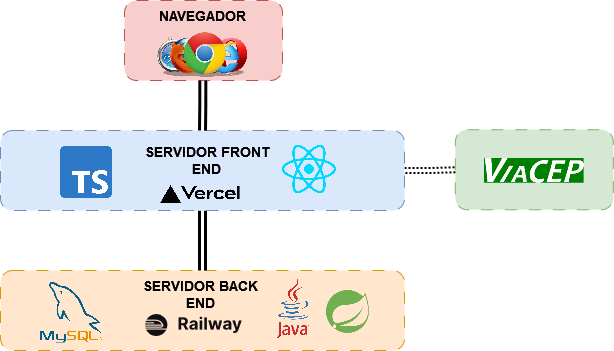
\includegraphics[width=0.8\textwidth]{images/EstruturaVocco(1).png}
        \caption{Arquitetura da aplicação}
        \label{arquitetura}
    \end{figure}

A seguir detalharemos cada uma das tecnologias escolhidas e como será feita a comunicação entre elas.

\subsection{Back-End}
No que diz respeito ao \textit{back-end}, adotamos o \textit{framework} \textbf{Spring Boot} em conjunto com a arquitetura \ac{msc}. O Spring Boot é uma escolha popular para o desenvolvimento de aplicativos Java devido à sua facilidade de configuração e rápida inicialização, como discutido nas Subseçõs 5.1.1 e 5.1.2 do Capítulo \ref{escolhas-descartes}. A arquitetura \ac{msc} divide a aplicação em três camadas distintas: \textbf{Model}, onde definimos as entidades e regras de negócio; \textbf{Service}, responsável pela lógica de negócio e manipulação dos dados; e \textbf{Controller}, que recebe as requisições \ac{http} e coordena a interação entre o cliente e o servidor. 

Além das camadas Model, Service e Controller, também implementamos a camada \textbf{Repository} como parte da arquitetura \ac{msc}. A camada Repository é responsável pela interação com o banco de dados, encapsulando a lógica de acesso e manipulação dos dados. Utilizando interfaces e métodos específicos, o Repository abstrai as operações \ac{crud}, permitindo que as demais camadas da aplicação interajam com o banco de dados de forma desacoplada e eficiente.

A utilização da arquitetura em camadas proporcionou diversos benefícios para o projeto. Em primeiro lugar, a separação de responsabilidades entre as camadas Model, Service, Controller e Repository facilitou a organização e compreensão do código-fonte, tornando-o mais legível e manutenível. Cada camada possui um propósito claro e bem definido, o que simplifica o processo de desenvolvimento e permite que diferentes equipes ou desenvolvedores trabalhem de forma independente em áreas específicas da aplicação.

\subsubsection{Gerenciamento de dependências}
Para o gerenciamento de dependências do projeto, optamos pelo \textbf{Maven}. Esta escolha se baseia nos inúmeros benefícios oferecidos por essa ferramenta. O Maven simplifica a gestão de dependências, permitindo que as bibliotecas necessárias sejam facilmente adicionadas ao projeto através de seu arquivo de configuração padrão (pom.xml). Além disso, o Maven automatiza tarefas como compilação, empacotamento e distribuição do projeto, tornando o processo de desenvolvimento mais eficiente e menos propenso a erros. Sua vasta gama de plugins oferece funcionalidades adicionais, como integração com ferramentas de teste e análise de código, promovendo uma abordagem mais completa para o desenvolvimento de \textit{software}. 

\subsection{Front-End}
Nesse projeto, optamos por utilizar \textbf{React} em conjunto com \textbf{TypeScript} para o desenvolvimento do \textit{front-end}. Essa escolha foi motivada pela necessidade de construir uma interface de usuário dinâmica e reativa, com uma base de código robusta e escalável, conforme discutido nas Subseções 5.1.3 e 5.1.4 do Capítulo \ref{escolhas-descartes}, onde são abordadas a adoção do TypeScript e a utilização do React para garantir produtividade, qualidade do código. O React é uma biblioteca JavaScript amplamente adotada que nos permite criar componentes reutilizáveis e composicionais, facilitando a construção de interfaces complexas de forma modular. Além disso, a integração com TypeScript adiciona um sistema de tipos estáticos ao JavaScript, oferecendo benefícios como detecção de erros em tempo de compilação e melhorando a manutenibilidade do código. A arquitetura baseada em componentes nos permitiu organizar a aplicação de forma hierárquica, facilitando a manutenção e o teste dos diferentes elementos da interface.

Na figura \ref{aplicação}, é possível ver o QRcode da aplicação que foi publicada na internet:

\begin{figure}[ht]
        \centering
        \href{https://vocco.vercel.app}{
\includegraphics[width=0.5\textwidth]{images/qrcode-url-aplicacao.png}}
        \caption{QRcode URL da Aplicação}
        \label{aplicação}
\end{figure}
\href{https://vocco.vercel.app}{https://vocco.vercel.app}

\newpage
\subsection{Banco de dados}
Em relação ao banco de dados,  optamos pelo \textbf{MySQL} devido à sua confiabilidade, desempenho e ampla adoção na indústria. O MySQL é um sistema de gerenciamento de banco de dados relacional que oferece recursos avançados de segurança e escalabilidade, sendo uma escolha sólida para aplicações de diferentes tamanhos e complexidades. Utilizamos o MySQL para armazenar e gerenciar os dados da aplicação, garantindo a integridade e disponibilidade das informações.


\subsubsection{Modelo Entidade Relacionamento}

O \ac{mer} é uma ferramenta fundamental no design de bancos de dados, pois permite visualizar de forma clara as relações entre as diversas entidades do domínio do sistema. O \ac{mer} da plataforma Vocco pode ser observado na Figura \ref{mer}.

\newpage
\begin{figure}[ht]
        \centering
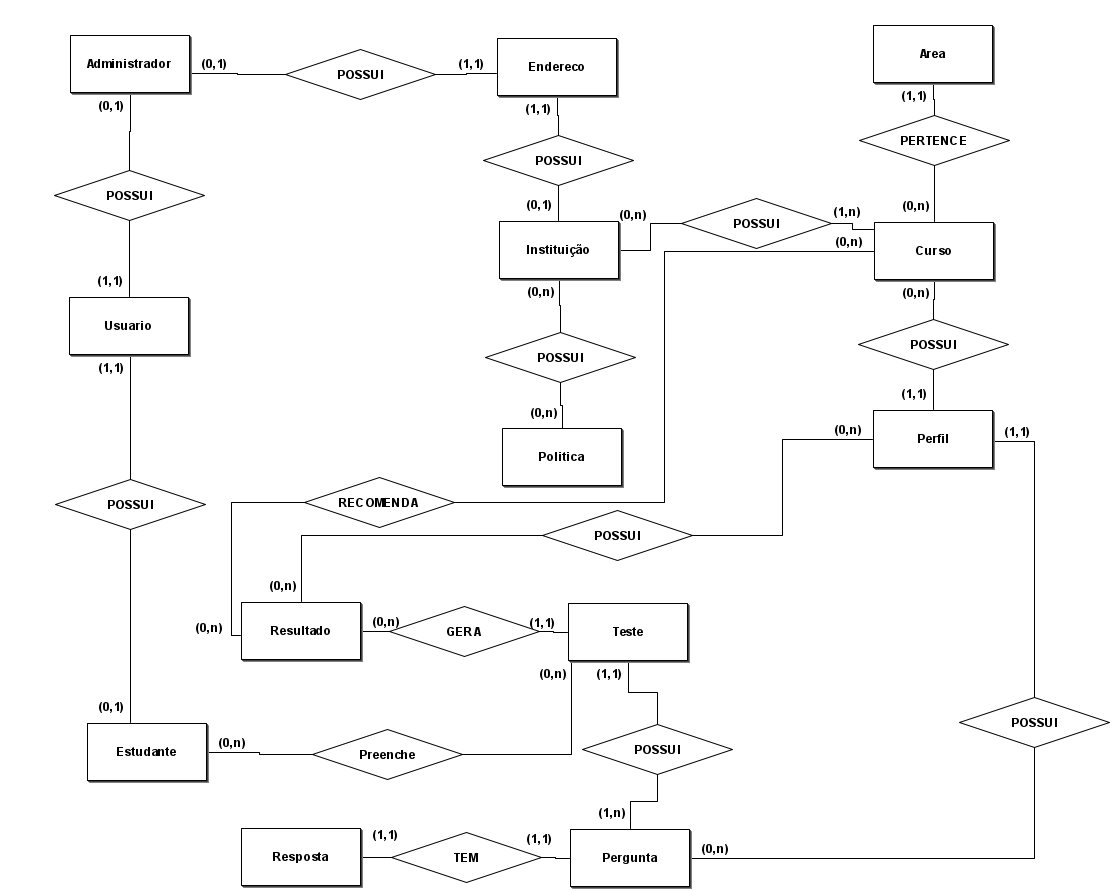
\includegraphics[width=1.0\textwidth]{images/mer.png}
        \caption{Modelo Entidade Relacionamento (MER) do projeto}
        \label{mer}
    \end{figure}
    
No processo de elaboração do diagrama, nosso foco primordial reside na visualização das relações entre as tabelas. Esse enfoque nos capacitou a estabelecer um sistema com informações confiáveis e interligadas, fundamentais para garantir a integridade e a eficácia dos dados. 

\newpage

\subsubsection{Diagrama Entidade Relacionamento}

O \ac{der} é uma ferramenta muito importante na modelagem de dados. Ele oferece uma visão clara das entidades, seus atributos e como elas se relacionam. Uma técnica central no \ac{der} é o uso de chaves estrangeiras para mapear as relações entre tabelas. Essas chaves garantem a integridade referencial entre os dados, assegurando que cada registro em uma tabela relacionada possa ser corretamente associado a outro em uma tabela diferente. O \ac{der} da plataforma Vocco pode ser observado na Figura \ref{der}

\begin{figure}[ht]
        \centering
        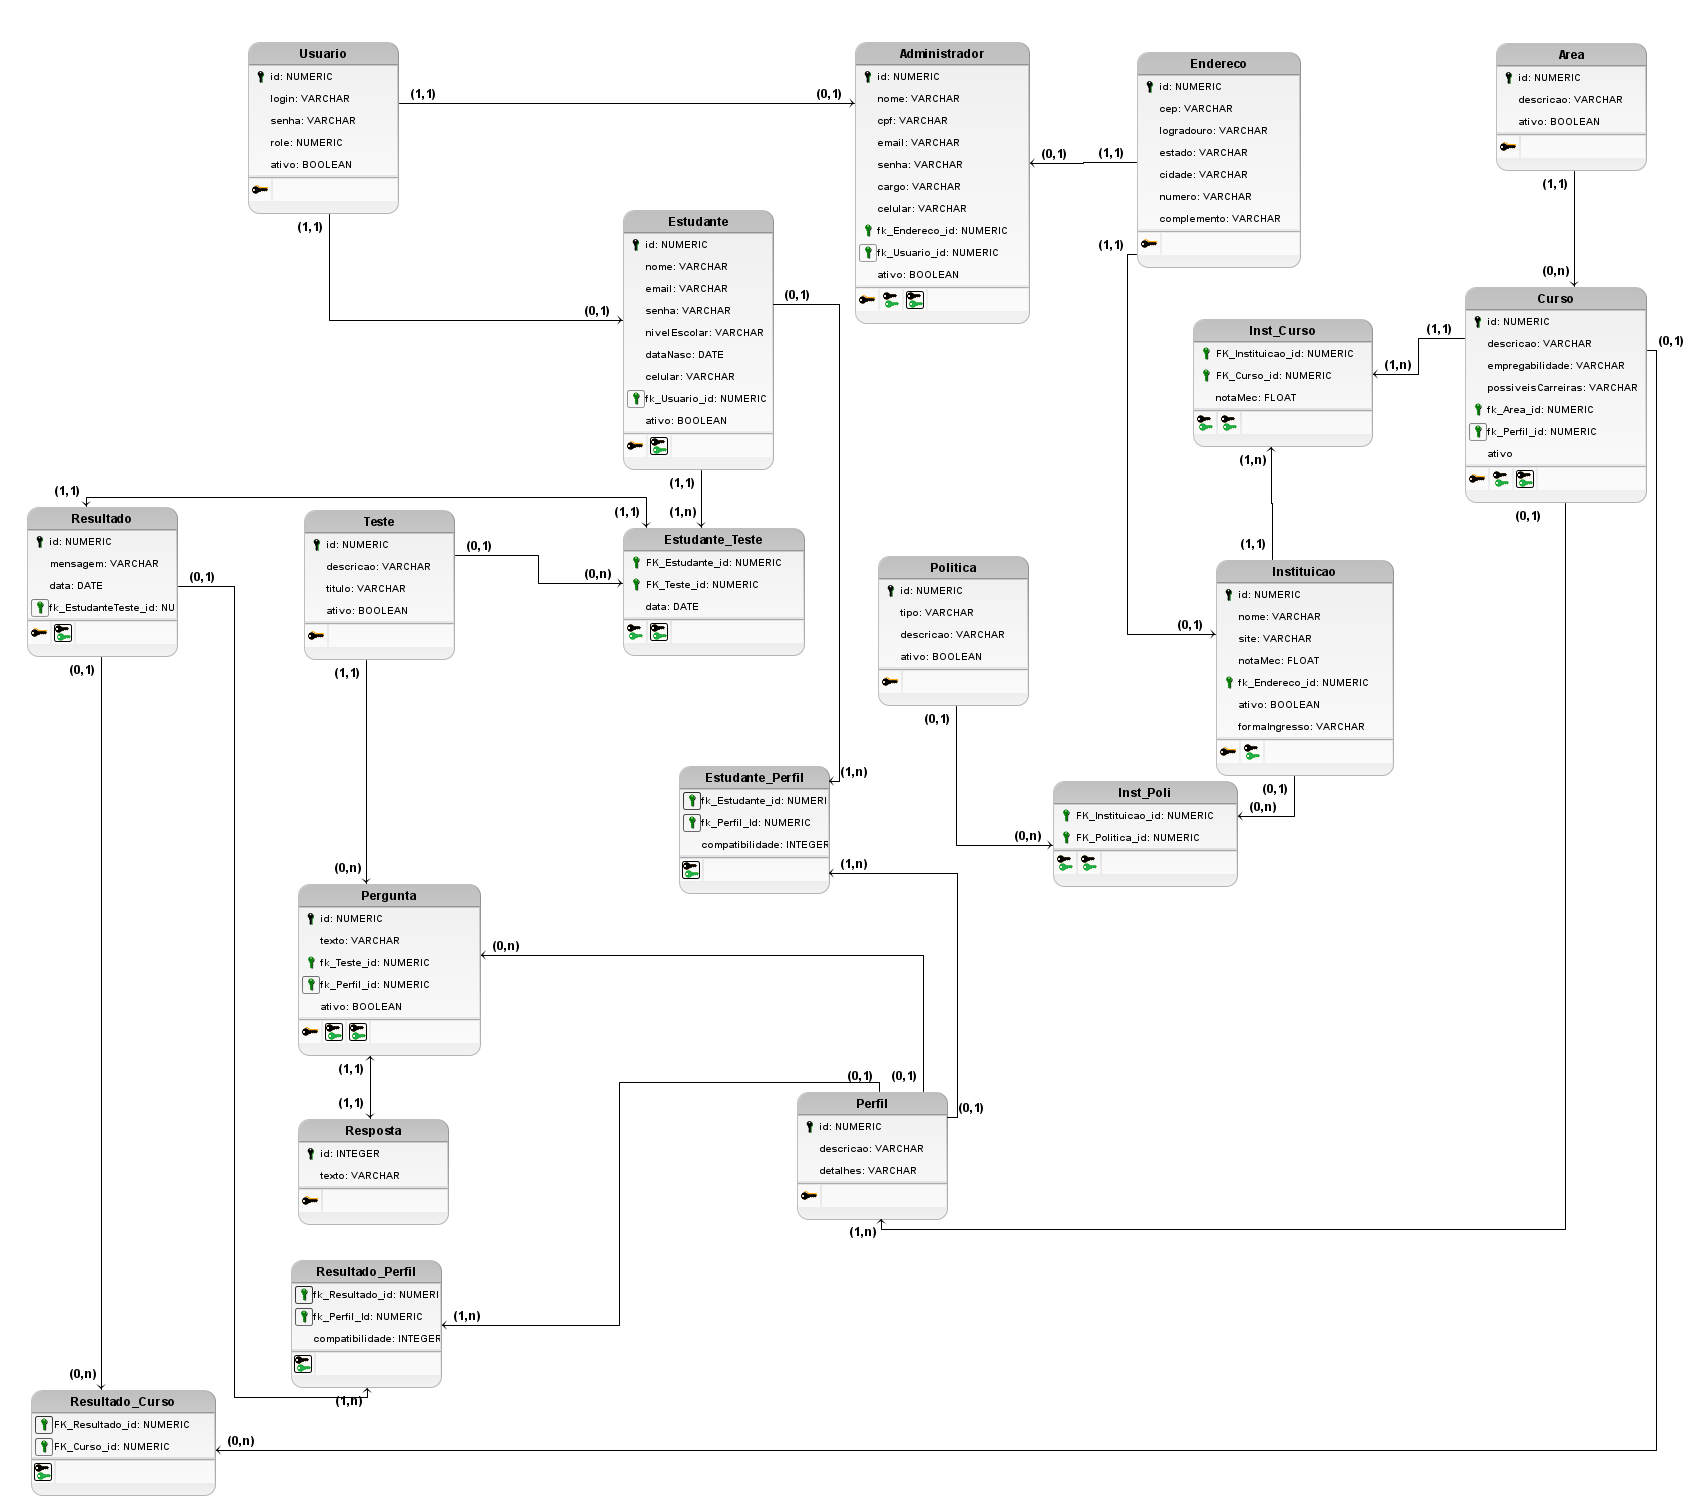
\includegraphics[width=1.0\textwidth]{images/der.png}
        \caption{Diagrama Entidade Relacionamento (DER) do projeto}
        \label{der}
    \end{figure}
    
Este diagrama oferece uma visão clara do processo de mapeamento dos relacionamentos entre as tabelas do banco de dados. Seguimos um padrão que envolve a criação de entidades associativas para representar os relacionamentos N-N. Para os relacionamentos 1-N, adicionamos a chave estrangeira na tabela que recebe o 'N' no mapeamento. Quanto aos relacionamentos 1-1 e 0-1, a escolha da tabela que recebe a chave estrangeira foi feita com base no que a equipe considerou mais relevante, levando em conta os requisitos específicos da plataforma.

\subsection{Integrações}
Para aprimorar a experiência do usuário e garantir a precisão dos dados de endereço nos cadastros, optamos por integrar a \ac{api} do \textbf{ViaCEP}. Essa integração permite que, ao preencher os campos de endereço em formulários de cadastro, o sistema automaticamente consulte a \ac{api} do ViaCEP para obter informações detalhadas, como rua, bairro, cidade e estado, com base no \ac{cep} fornecido pelo usuário. Essa abordagem simplifica e agiliza o processo de preenchimento dos cadastros, além de garantir a consistência e atualização dos dados de endereço. Ao utilizar essa \ac{api}, estamos priorizando a precisão e a eficiência na coleta e manipulação das informações de endereço, proporcionando uma experiência mais fluida e intuitiva para os usuários.

\subsection{Infraestrutura}
Por fim, para hospedar nosso projeto, optamos por utilizar serviços de hospedagem em nuvem para abrigar tanto o \textit{front-end} quanto o \textit{back-end}. Essa escolha foi motivada por diversos fatores que visam garantir uma maior eficiência e escalabilidade do sistema.

Primeiramente, a hospedagem em nuvem oferece uma infraestrutura altamente flexível, permitindo ajustes rápidos de recursos conforme a demanda do aplicativo. Além disso, ela proporciona uma maior disponibilidade e confiabilidade, com garantias de tempo de atividade elevado e redundância de dados. A facilidade de implementação e gerenciamento também foi considerada, já que a infraestrutura em nuvem permite uma rápida implantação e manutenção simplificada do sistema.

Por fim, os custos operacionais são otimizados, pois os serviços em nuvem geralmente seguem um modelo de pagamento conforme o uso, evitando gastos excessivos com infraestrutura desnecessária.

\subsection{Front - End}
Para hospedar o \textit{front-end}, escolhemos a plataforma \textbf{Vercel}, conhecida por sua facilidade de uso e escalabilidade. O \textit{front-end} foi desenvolvido com React e TypeScript, aproveitando os benefícios de uma tipagem estática para garantir um código mais robusto e menos propenso a erros. O uso do Vite como \textit{bundler} permitiu um processo de desenvolvimento mais rápido e eficiente, gerando builds otimizados e facilitando a implementação de novas funcionalidades. 

Além disso, é importante destacar que o \textit{front-end} se conecta ao \textit{back-end} através de requisições \ac{https}, garantindo a segurança e integridade dos dados transmitidos entre as partes. Essa abordagem assegura uma comunicação confiável e protegida entre os diferentes componentes do sistema, contribuindo para uma experiência segura e estável para os usuários.

\subsubsection{Back - End}
Para hospedar o \textit{back-end}, foi escolhida a plataforma \textbf{Railway}, conhecida por sua eficiência e facilidade de integração. Para o gerenciamento do banco de dados, optamos pelo MySQL, um sistema robusto e amplamente utilizado. A integração entre o Spring Boot e o MySQL foi facilitada através de um container Docker, gerado automaticamente pela plataforma Railway, proporcionando uma configuração que garante a conexão eficiente entre o \textit{core} da nossa aplicação e os dados persistidos, sendo que a conexão entre a aplicação e o banco foi realizada utilizando variáveis de ambiente definidas dentro do Railway, aumentando a segurança e confiabilidade. 



\subsection{Escalabilidade}
A escalabilidade é crucial para garantir que a Vocco possa se adaptar ao crescimento de forma eficaz, mantendo flexibilidade, confiabilidade, eficiência e manutenibilidade. Acreditamos  que tais metas serão alcançadas por meio de nossas decisões de utilizar serviços em nuvem e um sistema gerenciador de banco de dados que facilite o processo de expansão do nosso sistema. Neste momento, nosso foco está em manter uma \textbf{escalabilidade vertical}, o que implica em aumentar a capacidade de armazenamento em vez de adicionar mais servidores. Essa abordagem nos permite otimizar recursos e simplificar o gerenciamento, garantindo que Vocco possa se adaptar ao crescimento de maneira ágil e econômica.
\subsection{Controle de versão}
 No desenvolvimento deste projeto, optamos por utilizar tanto o \textbf{Git} como o \textbf{GitHub} para o controle de versão do código-fonte. O Git foi escolhido como sistema de controle de versão devido à sua eficiência e robustez no gerenciamento de alterações de código, permitindo o acompanhamento do histórico de modificações, a colaboração entre os membros da equipe e a criação de branches para o desenvolvimento de novas funcionalidades de forma isolada. Além disso, o GitHub foi utilizado como plataforma de hospedagem remota dos repositórios Git, proporcionando uma maneira conveniente de compartilhar o código entre os membros da equipe, revisar alterações, gerenciar problemas e automatizar processos de \ac{ci} e \ac{cd}.

 Na figura \ref{github}, é possível acessar o nosso repositório do GitHub do projeto: 

\begin{figure}[ht]
        \centering
        \href{https://github.com/betatrix/Projeto-Integrado-I}{
        
\includegraphics[width=0.5\textwidth]{images/qrcode-repo-github.png}
        }
        \caption{QRcode Repositório do GitHub}
        \label{github}
\end{figure}
 
 A utilização do Git e do GitHub garante que os membros da equipe colaborem de maneira eficaz e organizada, mantendo o código atualizado e permitindo uma gestão eficiente das tarefas e do progresso do projeto.

\section{Manutenibilidade}

A manutenibilidade de um \textit{software} refere-se à facilidade com que ele pode ser mantido e modificado ao longo do tempo. Em outras palavras, é a capacidade do sistema de ser compreendido, adaptado, corrigido e aprimorado de maneira eficiente e econômica. A manutenibilidade é uma característica fundamental de qualidade do \textit{software}, pois afeta diretamente a capacidade da equipe de desenvolvimento de responder a novos requisitos, corrigir falhas e melhorar a funcionalidade do sistema ao longo do ciclo de vida do \textit{software}.

\subsection{Code Convention}
A adoção de convenções de código padronizadas é fundamental para garantir a legibilidade, consistência e manutenção eficiente do software. Este capítulo aborda as práticas recomendadas e as diretrizes específicas que devem ser seguidas por todos os desenvolvedores do projeto ao escrever e revisar o código.

\begin{itemize}
    \item \textbf{Back-End}
     Seguiremos as convenções de código  para a linguagem Java conforme estabelecidas na documentação oficial da Oracle. Algumas das principais orientações incluem:
     \begin{itemize}
        \item \textbf{Nomenclatura de Classes, Interfaces e Tipos:}
        Utilizar PascalCase, começando com letra maiúscula;
        \item \textbf{Nomenclatura de Métodos e Variáveis:}
        Utilizar camelCase, começando com letra minúscula;
        \item \textbf{Constantes e variáveis:}
        Utilizar letras maiúsculas separadas por sublinhados;
        \item \textbf{Indentação:}
        Utilizar quatro espaços para indentação e evitar o uso de tabulação;
        \item \textbf{Comentários:}
        Explicar trechos de código complexos ou documentar \ac{api};
        \item \textbf{Linhas de Comprimento:}
         Limitar o comprimento a 80-100 caracteres para melhorar a legibilidade;
        \item \textbf{Imports:}
        Evitar importar pacotes inteiros, trazendo apenas classes específicas ou utilizar asterisco apenas para \textit{imports} estáticos.
     \end{itemize}
\end{itemize}
\begin{itemize}
    \item \textbf{Front-End}
     Para o desenvolvimento \textit{front-end}, adotaremos as principais convenções de código:
     \begin{itemize}
        \item \textbf{Nomenclatura de variáveis:}
        Utilizaremos camelCase, começando com letra minúscula;
        \item \textbf{Nomenclatura de funções:}
        Utilizaremos PascalCase, começando com letra maiúscula;
        \item \textbf{Declaração de variáveis:}
        Preferimos utilizar \textbf{let} ou \textbf{const} em vez de \textbf{var} para declarar variáveis, pois isso ajuda a evitar problemas de escopo;
        \item \textbf{Convenções de nome para constantes:}
        Nomearemos constantes utilizando letras maiúsculas e palavras separadas por sublinhados;
        \item \textbf{Comentários:}
        Faremos uso de comentários para documentar o código, explicando o propósito de funções e partes importantes do código;
        \item \textbf{Tratamento de erros:}
        Faremos uso de blocos try-catch para capturar e lidar com exceções, quando necessário;
        \item \textbf{Ponto e vírgula:}
         Apesar de o JavaScript permitir a omissão de ponto e vírgula no final das declarações, incluiremos sempre para evitar comportamentos inesperados;
        \item \textbf{Uso de aspas:}
        Utilizaremos aspas duplas de forma consistente para \textit{strings}.
 
     \end{itemize}
\end{itemize}
\subsection{Ferramentas de testes}

Os testes de \textit{software} são uma etapa fundamental no ciclo de desenvolvimento de \textit{software}, cujo objetivo é garantir a qualidade e a confiabilidade do produto final. Essas atividades consistem em verificar se o \textit{software} atende aos requisitos estabelecidos, se funciona corretamente em diferentes cenários de uso e se está livre de defeitos e erros. Os testes de \textit{software} podem abranger diversas áreas, como funcionalidade, desempenho, segurança e usabilidade, e são conduzidos por meio de técnicas e ferramentas específicas. 

Para a realização dos testes utilizaremos as seguintes ferramentas:
 
\begin{itemize}
    \item \textbf{JUnit:}
     Será utilizado no \textit{back-end} o \textit{framework} JUnit como ferramenta de testes automatizados. Ele oferece recursos que facilitam a criação e execução de testes, incluindo suporte para testes parametrizados, testes de exceção e integração com ferramentas que utilizaremos para o desenvolvimento.
    \item \textbf{Jest:}
    Para os testes automatizados no \textit{front-end}, escolhemos o Jest como nossa ferramenta principal. Ele abrange uma ampla gama de cenários de teste, desde os unitários mais simples até os de integração mais complexos, destacando-se pela sua facilidade e rapidez de uso. 
    \item \textbf{Typescript EsLint:}
    Para conduzir uma análise estática abrangente em nosso \textit{front-end}, decidimos adotar o TypeScript ESLint. Essa escolha se deve ao fato de que essa ferramenta combina as vantagens de \textit{linting} de código, e nos permite definir regras personalizadas, garantindo que sigamos as melhores práticas e padrões de codificação estabelecidos.
    \item \textbf{SonarQube:}
    Utilizaremos o SonarQube como nossa ferramenta de análise estática do \textit{back-end}. Ele realiza uma avaliação detalhada do código, identificando potenciais problemas, vulnerabilidades de segurança, \textit{bugs}, duplicações de código e padrões de código não conformes.
\end{itemize}
\subsection{Design Patterns}
Optamos por adotar o padrão \textbf{SOLID} como base para o desenvolvimento deste sistema, pois ele encapsula um conjunto de cinco princípios essenciais de design de software, idealizados por Robert C. Martin. Esses princípios são fundamentais para criar um código mais limpo, modular e fácil de manter. Ao seguirmos esses princípios, garantimos que nossas classes e módulos tenham responsabilidades bem definidas, promovendo a coesão e o baixo acoplamento, o que facilita tanto a compreensão do código quanto sua manutenção no futuro. 

Também utilizaremos o padrão \ac{dto} para permitir a comunicação eficiente de dados entre diferentes partes do nosso sistema. Para representar esses objetos de transferência de dados, optaremos por utilizar \textit{\textbf{records}}, aproveitando as suas vantagens de imutabilidade e clareza.

\section{Segurança, Privacidade e Legislação}
A segurança representa um aspecto essencial na arquitetura da Vocco. Dessa forma, nesta seção serão citadas as boas práticas e tecnologias usadas para garantir uma maior confiabilidade e segurança para os usuários de nossa aplicação.

\subsection{Lei Geral de Proteção de Dados (LGPD)}
A \ac{lgpd} (Congresso Nacional, 2018), foi promulgada com o objetivo de proteger os direitos fundamentais de liberdade e de privacidade, e a livre formação da personalidade de cada indivíduo, atuando sobre o tratamento de dados pessoais, incluindo em meios digitais.
Com isso, durante o planejamento da estruturação da plataforma, foram definidas ações visando atender a essas necessidades de segurança, para dessa forma assegurar que a aplicação estivesse em conformidade com essa legislação e atendendo ao compromisso de proteger nossos usuários.

A aplicação respeita o livre acesso a esses dados, definido no Art. 6\textsuperscript{o},IV, e requisitará consentimento dos usuários para armazenar os dados fornecidos, o que confere a ela conformidade com o Art. 7\textsuperscript{o}
,I.


\subsection{Autenticação e Autorização}
A aplicação conta com etapas de autenticação e autorização à depender do usuário e seus privilégios, para garantir maior privacidade à informações e também uma melhor gestão de como os recursos serão acessados tanto no \textit{back-end} como no \textit{front-end}.

A autenticação como sendo o login do usuário no sistema e a autorização como sendo o processo posterior, em que é verificado se o usuário tem permissão de acesso a um determinado recurso.
O Spring Security é um \textit{framework} do Java que possui um sistema  de autenticação e autorização para aplicações Java, como é o caso da Vocco, além disso conta com proteção contra ataques como \textit{session fixation}, \textit{clickjacking} e protege contra injeção de DDR, se mostrando uma ferramenta madura e qualificada para proteger a aplicação.

Para implementar o fluxo de autenticação, é usado o \textit{Bearer Token}, que é gerado após a validação das credenciais pelo \textit{back-end} Java Spring Boot, garantindo a autenticidade e evitando conflitos.
O \textit{Bearer Token} ou "token de portador", é um tipo de token de acesso usado para acessar recursos protegidos, como \ac{api}. Esse \textit{token} é gerado pelo servidor em resposta a uma solicitação de login, e deve ser incluído no cabeçalho de autorização das solicitações \ac{http} para recursos protegidos.


\subsection{Criptografia de Dados}
A criptografia é uma alternativa ideal para anonimização de dados, reduzindo as chances de violação de dados e as multas que a \ac{lgpd} pode impor. Desempenha um papel fundamental na proteção das informações, tornando-as ininteligíveis para terceiros não autorizados, impedindo que pessoas não autorizadas utilizem as informações para benefício próprio, embaralhando os dados de forma que não sejam legíveis, tanto por humanos quanto por sistemas projetados para interpretar informações.

Para aplicar essa medida de segurança na aplicação Vocco, será usada a ferramenta \textbf{BCrypt}, que tem o intuito de esconder senhas criadas pelos usuários em forma de texto “puro” em dados indecifráveis, utilizando o algoritmo \textit{hash}.
Será utilizada essa ferramenta para criptografar as senhas dos usuários no banco de dados. 


\section{Viabilidade Financeira}
A análise da viabilidade financeira demonstra o custo operacional estimado para o primeiro ano após o lançamento da plataforma. Esta avaliação considera os custos de mão de obra de desenvolvimento, registro de domínio, utilização dos serviços oferecidos pela plataforma de desenvolvimento na nuvem Railway para hospedar o \textit{back-end}, levando em conta um aumento de 30\% no processamento e uso dos recursos da mesma e também pela utilização da plataforma Vercel para hospedar o \textit{front-end}. Com base nesses parâmetros, segue a estimativa dos custos operacionais para o primeiro ano após o lançamento da plataforma.

\begin{table}[h!]
\centering
\caption{Estimativa dos Custos Operacionais}
\begin{tabular}{|m{5cm}|m{4cm}|m{4cm}|}
\hline
\textbf{Descrição}   & \textbf{Valor Anual (R\$)} & \textbf{Valor Mensal (R\$)} \\
\hline
Custo de Desenvolvimento & 42.240,00 & 3.520,00 \\
\hline
Registro de Domínio & 40,00 & 3,33 \\
\hline
Plataforma Railway & 702,92 & 58,58 \\
\hline
Plataforma Vercel & 1.225,2  & 102,10 \\
\hline
\textbf{Total} & \textbf{44.208,12} & \textbf{3.684,01} \\
\hline
\end{tabular}
\label{table:estimativa-custos}
\\[1ex]
\footnotesize \textbf{Fonte}: Elaborado pelo autor.
\end{table}

A estimativa dos custos operacionais detalhada, apresenta que o Custo de Desenvolvimento anual será calculado com base em 1.320 horas anuais de trabalho, cumpridas por uma gerente e quatro desenvolvedoras. A gerente será remunerada em R\$8,00 por hora, enquanto cada desenvolvedora será remunerada em R\$6,00 por hora. O valor de registro de domínio será de R\$40,00 o qual é uma taxa paga anualmente. Além disso, há o custo com a plataforma Railway em que são considerados os valores de utilização do plano mensal Hobby de R\$ 25,33, mais o valor adicional de R\$ 398,96 para o aumento de 30\% no uso dos recursos da plataforma, e esse valor é dividido em 12 meses. Por fim,  o custo com a plataforma Vercel será de R\$102,10 com o plano mensal Pró. Esses valores são apresentados  na Tabela \ref{table:detalhamento-custos} a seguir:

\begin{table}[h!]
\centering
\caption{Detalhamento dos Custos Operacionais}
\begin{tabular}{|m{4cm}|m{4cm}|m{3cm}|m{3cm}|}
\hline
\textbf{Item} & \textbf{Descrição} & \textbf{Valor Anual (R\$)} & \textbf{Valor Mensal (R\$)} \\
\hline
Desenvolvimento & 1 Gerente  & 10.560,00 & 880,00 \\
\hline
 Desenvolvimento & 4 Desenvolvedoras & 31.680,00 & 2.640,00 \\
\hline
Registro de Domínio & Plano Fixo Anual & 40,00 & 3,33 \\
\hline
Plataforma Railway & Plano mensal Hobby & 303,96 & 25,33 \\
\hline
Plataforma Railway & 30\% de uso adicional & 398,96 & 33,25 \\
\hline
Plataforma Vercel & Plano Pró & 1.225,20 & 102,10 \\
\hline
\textbf{Total} & & \textbf{44.208,12} & \textbf{3.684,01} \\
\hline
\end{tabular}
\label{table:detalhamento-custos}
\\[1ex]
\footnotesize \textbf{Fonte}: Elaborado pelo autor.
\end{table}

Dessa forma, a estimativa de Custo Operacional anual será de R\$44.208,12 e mensal de R\$3.684,01, como apresentado nas tabelas anteriores.


\subsection{Monetização}

A plataforma oferecerá suas funcionalidades gratuitamente, visando garantir a acessibilidade e engajamento dos usuários, porém apresentará campos com anúncios, com o intuito de cobrir os custos operacionais e sustentar o desenvolvimento contínuo. Dessa forma, a estratégia de monetização planejada envolve o estabelecimento de parcerias com cursos pré-vestibular visando que a receita gerada cubra os custos necessários. 

A monetização será feita a partir de anúncios e conteúdo patrocinado, provenientes inicialmente de seis empresas de cursos pré-vestibular. O valor cobrado estimado será composto por uma taxa fixa de R\$ 600,00 e por uma comissão de 1,5\% sobre as vendas realizadas através dos \textit{links} disponibilizados na plataforma, considerando o valor médio de R\$ 253,00 em cada curso vendido. Os valores totais são apresentados na Tabela \ref{table:estimativa-receitas} a seguir: 

\begin{table}[h!]
\centering
\caption{Estimativa de Receitas Operacionais}
\begin{tabular}{|m{6cm}|m{4cm}|m{4cm}|}
\hline
\textbf{Descrição} & \textbf{Valor Anual (R\$)} & \textbf{Valor Mensal (R\$)} \\
\hline
Receita Fixa de Anúncios & 43.200,00 & 3.600,00 \\
\hline
Comissão de Vendas (1,5\% sobre vendas) & 2.736,00 & 228,00 \\
\hline
\textbf{Total de Receita} & \textbf{45.936,00} & \textbf{3.828,00} \\
\hline
\end{tabular}
\label{table:estimativa-receitas}
\\[1ex]
\footnotesize \textbf{Fonte}: Elaborado pelo autor.
\end{table}

Levando em consideração uma base estimada de 1.000 usuários ativos mensalmente e assumindo uma taxa de conversão de 1\% desses usuários em vendas efetivas, projetamos uma receita mensal fixa no valor de R\$ 3.600,00 e comissão de vendas no valor de R\$ 228,00. Dessa forma, a estimativa total de receita anual será de R\$ 45.936,00 e mensal de R\$ 3.828,00, como foi apresentado pela Tabela \ref{table:estimativa-receitas}.


\section{Fases de Entrega}

As fases de entrega delimitam as datas das principais entregas do sistema para a disciplina, sendo elas a Prova de Conceito, o Produto Mínimo Viável e o Produto Final.

\subsection{ Prova de Conceito (POC)}

Para a prova de conceito desenvolvemos o requisito de manutenção das \ac{ies} cadastradas na plataforma Vocco, concebida como uma parte essencial do produto final planejado. Destinada aos administradores do sistema, essa funcionalidade foi desenvolvida para proporcionar uma gestão eficiente das instituições de ensino cadastradas, englobando desde o cadastro até associações com cursos e políticas públicas. 

As funcionalidades entregues foram:

\begin{itemize}
    \item \textbf{Tela inicial}: Tela disponibilizada para o administrador gerenciar as entidades da aplicação.
    \item \textbf{Cadastro}: Incluir informações sobre a instituição. 
    \item \textbf{Listagem}: Visualizar todas as instituições ativas e inativas.
    \item \textbf{Detalhamento}: Acessar informações específicas de cada instituição.
    \item \textbf{Alteração}: Modificar dados cadastrais conforme necessário.
    \item \textbf{Exclusão}: Implementamos exclusão lógica, definindo o campo 'ativo' como falso. 
    \item \textbf{Associação com Curso}: Vincular instituições a cursos específicos.
    \item \textbf{Associação com Política Pública}: Integrar instituições às políticas de entrada e permanência oferecidas.
\end{itemize}

 Os protótipos das telas desenvolvidas podem ser acessados no apêndice \ref{apendice_a}.


\subsection{Produto Mínimo Viável (MVP)}

Na entrega do MVP, além do que foi desenvolvido na \ac{poc}, será entregue a funcionalidade principal do sistema, que se trata do preenchimento do teste vocacional  bem como a recomendação dos cursos e áreas que mais se encaixam no perfil do estudante, a depender das respostas enviadas. Além disso, para essa funcionalidade ser entregue é necessário que o cadastro dos estudantes também já esteja implementado. Esta entrega será feita no mês de junho de 2024.


\subsection{Produto Final}

No Produto Final será entregue o projeto completo, contendo todas as funcionalidades propostas, como o teste vocacional, cadastro de administradores, cadastros de cursos e áreas, disponibilização das informações das Universidades estaduais do Estado de São Paulo, e as universidades Federais do Brasil, bem como todas as funcionalidades definidas anteriormente. É importante destacar que, durante o desenvolvimento do projeto, devido à sua complexidade e ao foco principal da aplicação, foi decidido descartar a integração com instituições estrangeiras que aceitam a nota do ENEM, conforme discutido na Seção 5.2 do Capítulo \ref{escolhas-descartes}. Esta entrega será feita no mês de dezembro de 2024.



\newpage

\section{Métricas}

Ao longo do desenvolvimento do projeto, o progresso foi acompanhado através de medições realizadas mensalmente tanto no repositório do projeto \textit{front-end} quanto no repositório do projeto \textit{back-end}. Conforme mostra o quadro foram analisados os itens: reuniões da equipe, posts no blog, vídeos no canal do youtube do projeto AdasTech, quantidade de requisitos, quantidade de entidades de Banco de Dados, Interfaces, classes, Tamanho do Projeto (em MegaBytes), quantidade de métodos, commits, Arquivos, linhas de código e informações sobre os testes unitários. De todos os elementos analisados na tabela abaixo, as informações sobre o número de classes, interfaces, métodos, atributos, arquivos e linhas de código, foram obtidas através da ferramenta MetricRunner. Os valores informados a cada mês são acumulativos.


\begin{figure}[ht]
        \centering
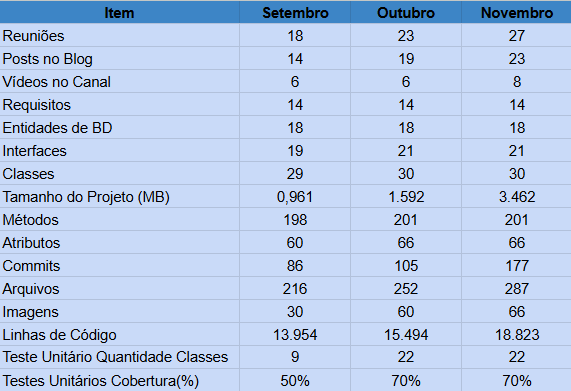
\includegraphics[width=0.85\textwidth]{images/tabela-metricas.png}
        \caption{Tabela de métricas do projeto primeiro semestre 2024}
        \label{fig:enter-label}
    \end{figure}
As métricas representam numericamente o andamento do projeto, demonstrando quais foram os períodos de maior atividade do grupo e o tamanho do projeto como um todo.

\newpage

\subsection{Ferramentas Auxiliares}

Com o intuito de simplificar o processo de análise do projeto como um todo, foi usada a ferramenta MetricRunner, que auxilia na contagem do número de classes, interfaces, métodos, atributos, arquivos e linhas de código do projeto Vocco.
Para fazer uso desta ferramenta é necessário cumprir os seguintes passos: 

1- Buscar no Maven Central a Biblioteca Reflections versão 0.9.9-RC1;

2- Adicionar a dependência da biblioteca indicada, no arquivo Pom;

3- Adicionar a classe MetricRunner à aplicação;

4- Alterar o valor da variável rootPackage para o nome do pacote raiz da aplicação;  

5- Executar a classe MetricRunner.


\subsection{Estatísticas do Projeto}

Para obtenção de elementos visuais, e mais informações estatísticas à respeito de ambos os projetos (\textit{back-end} e \textit{front-end}), foi utilizada a ferramenta GitStats para a geração de gráficos e tabelas informativas.


Na figura \ref{fig:dadosGeraisRepositorioBack}, são apresentados os dados gerais à respeito do repositório GitHub referente ao projeto \textit{back-end}.

\begin{figure}[ht]
        \centering
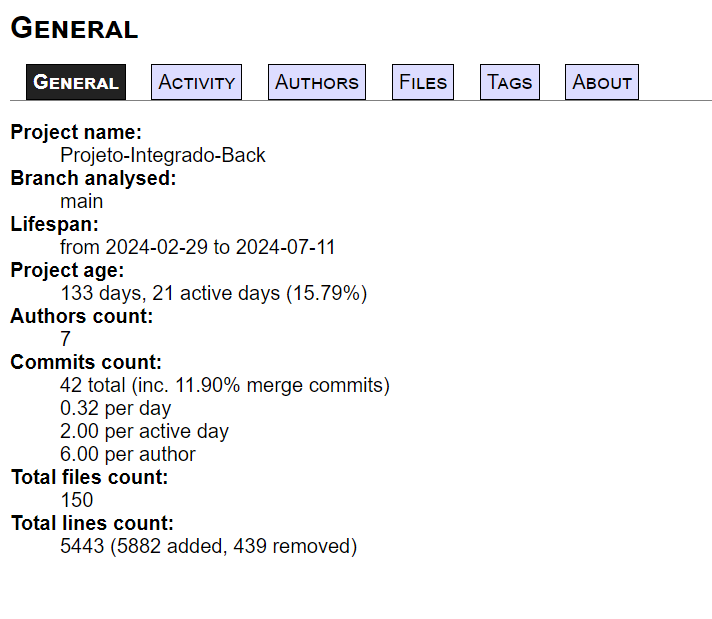
\includegraphics[width=0.65\textwidth]{images/dados-gerais-stats-back.png}
        \caption{Dados Gerais sobre o repositório \textit{back-end} do GitHub}
        \label{fig:dadosGeraisRepositorioBack}
    \end{figure}

\newpage

Na figura \ref{fig:dadosCommitsDiasBack} são apresentados os dados referentes à relação entre o dia da semana, e o horário em que foram feitos os commits no repositório do projeto \textit{back-end} do GitHub.

\begin{figure}[ht]
        \centering
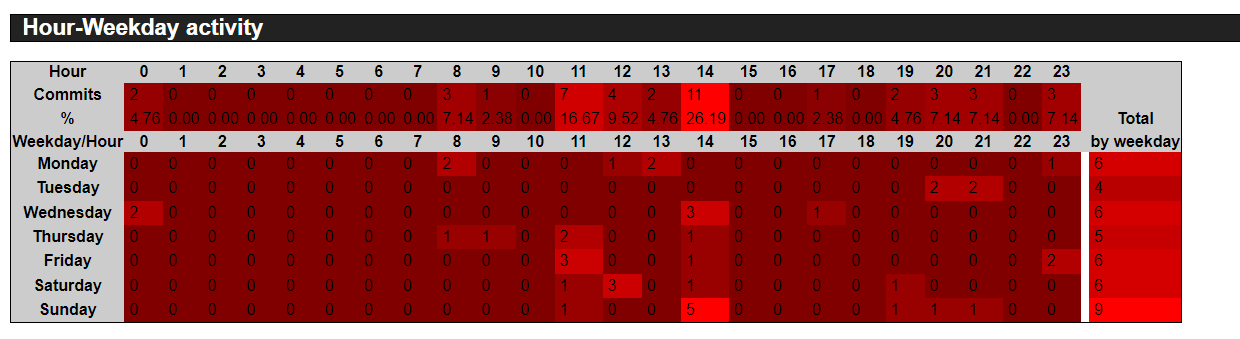
\includegraphics[width=1.0\textwidth]{images/commits-hora-semana-stats-back.png}
        \caption{Dados Gerais sobre o repositório \textit{back-end} do GitHub}
        \label{fig:dadosCommitsDiasBack}
    \end{figure}

Na figura \ref{fig:commitsBack} são apresentados os dados referentes ao número de commits em cada mês do ano de 2024 referente ao repositório do projeto \textit{back-end} do GitHub.

\begin{figure}[ht]
        \centering
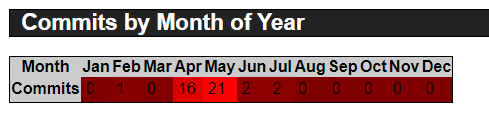
\includegraphics[width=0.75\textwidth]{images/commits-mes-stats-back.png}
        \caption{Número de commits em cada mês do ano de 2024}
        \label{fig:commitsBack}
    \end{figure}
    

Na figura \ref{fig:commitsAutorBack} são apresentados os dados referentes ao número de commits por autor no repositório do projeto \textit{back-end} do GitHub.  

\begin{figure}[ht]
        \centering
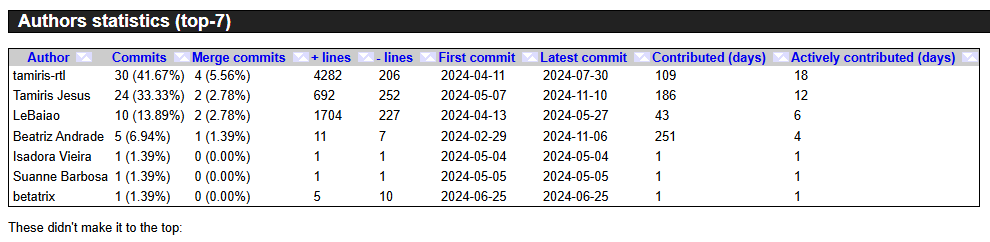
\includegraphics[width=1.0\textwidth]{images/autores-stats-back.png}
        \caption{Número de commits por autor}
        \label{fig:commitsAutorBack}
    \end{figure}

\newpage

Na figura \ref{fig:numeroLinhasBack} é apresentado o gráfico referente ao número de linhas de código adicionadas por autor no repositório do projeto \textit{back-end} do GitHub.  

\begin{figure}[ht]
        \centering
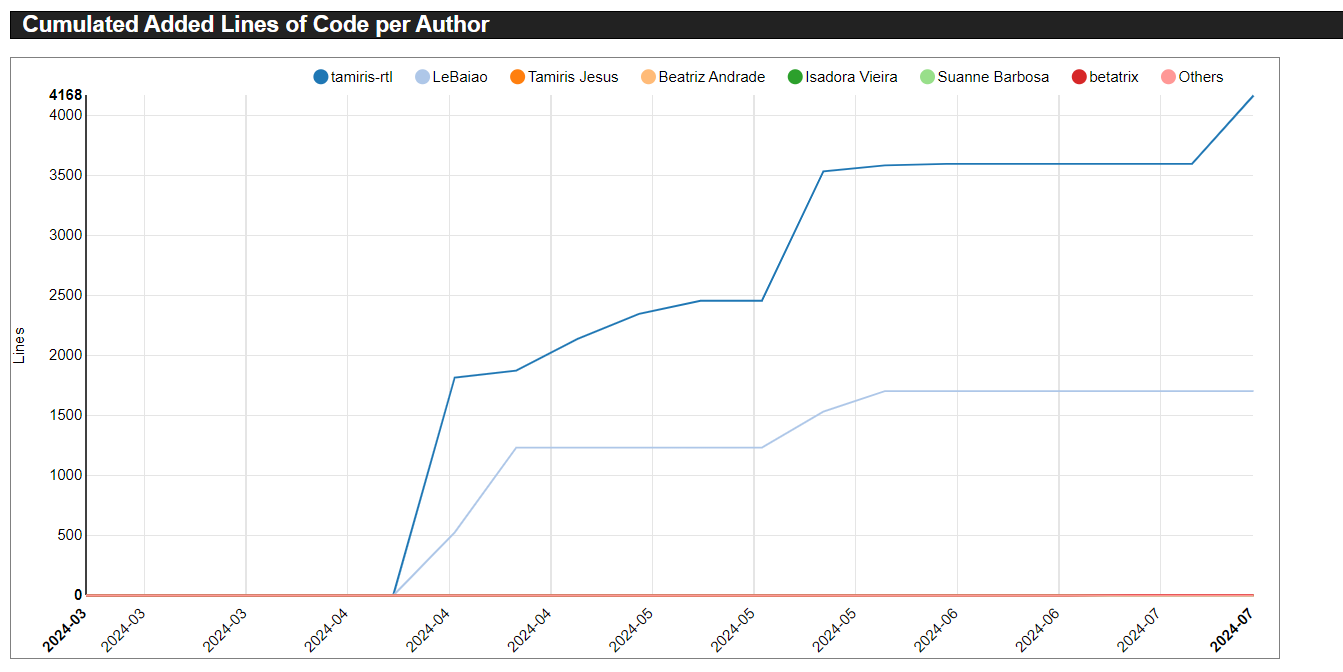
\includegraphics[width=1.0\textwidth]{images/linhas-por-autor-stats-back.png}
        \caption{Número de linhas de código por autor}
        \label{fig:numeroLinhasBack}
    \end{figure}



Na figura \ref{fig:linhasPorAutorBack} é apresentado o gráfico referente ao número de commits por autor no repositório do projeto \textit{back-end} do GitHub.  

\begin{figure}[ht]
        \centering
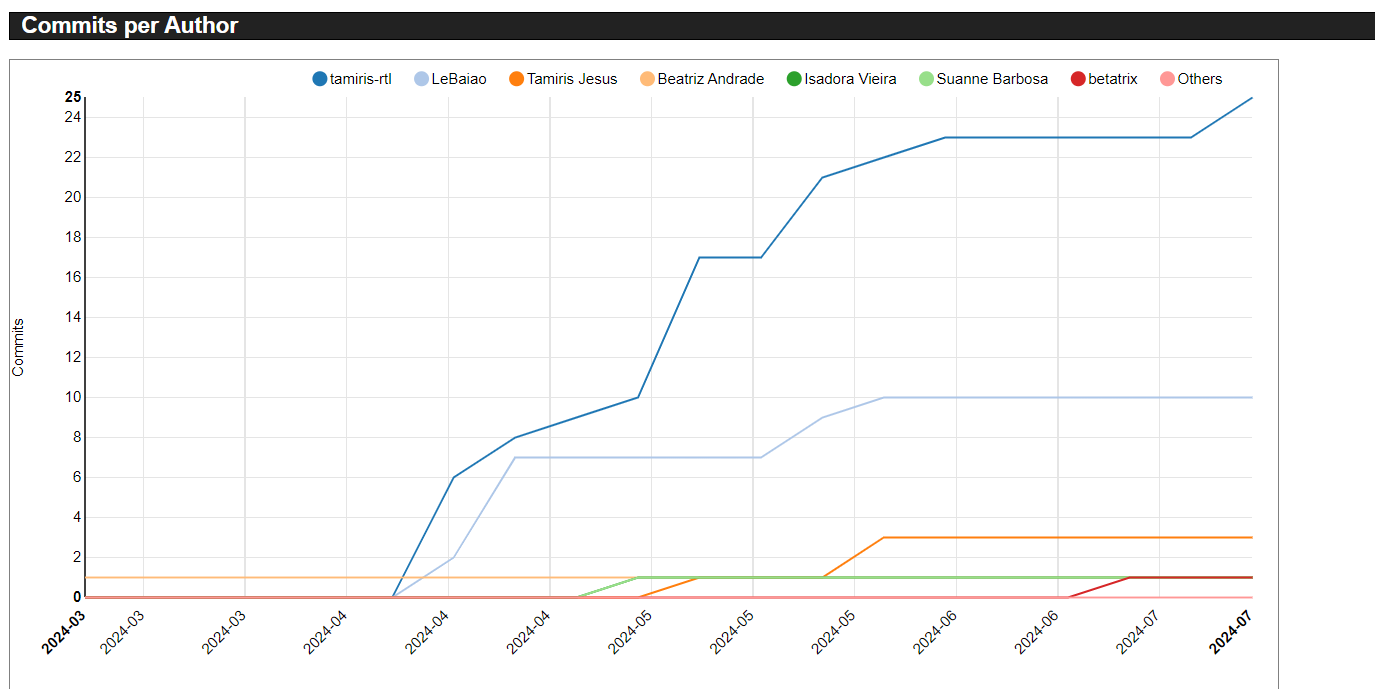
\includegraphics[width=1.0\textwidth]{images/commits-autor-stats-back.png}
        \caption{Gráfico número de commits por autor}
        \label{fig:linhasPorAutorBack}
    \end{figure}

\newpage

A figura \ref{fig:linhasPorAutor2Back} é um complemento do gráfico da figura 19, no qual é apresentado o gráfico referente ao número de commits por autor no repositório do projeto \textit{back-end} do GitHub.  

\begin{figure}[ht]
        \centering
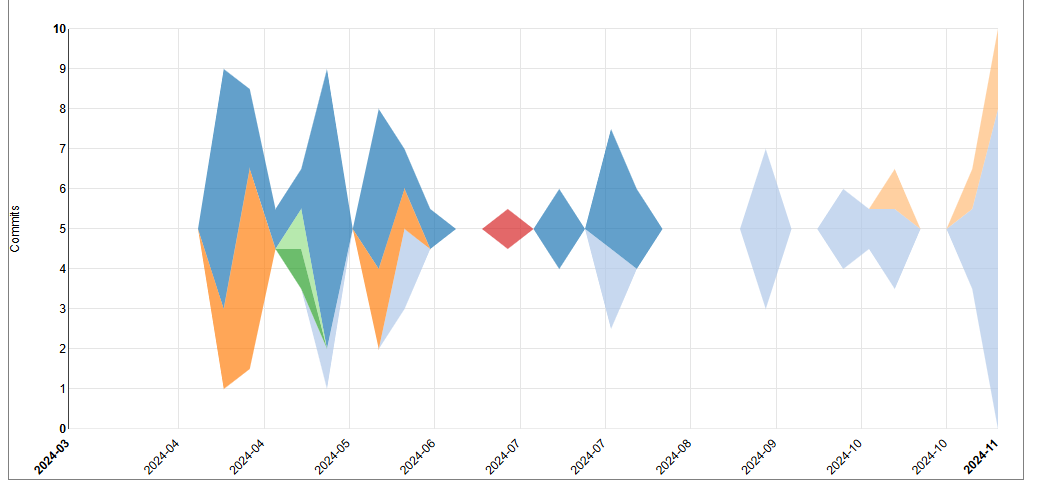
\includegraphics[width=1.0\textwidth]{images/commits-autor2-stats-back.png}
        \caption{Gráfico número de commits por autor}
        \label{fig:linhasPorAutor2Back}
    \end{figure}



Na figura \ref{fig:rankingAutoresBack} é apresentado o ranking dos autores com o maior número de commits em cada mês do ano de 2024 no repositório do projeto \textit{back-end} do GitHub.

\begin{figure}[ht]
        \centering
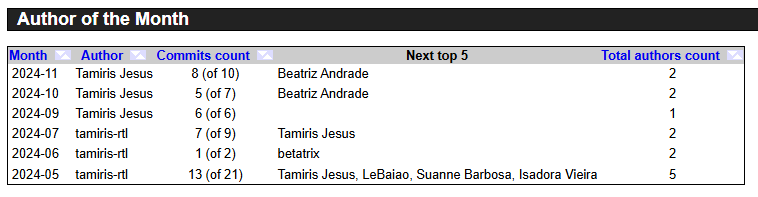
\includegraphics[width=1.0\textwidth]{images/rank-autor-stats-back.png}
        \caption{Tabela autor com o maior número de commits em cada mês do ano de 2024}
        \label{fig:rankingAutoresBack}
    \end{figure}

\newpage

Na figura \ref{fig:arquivosPorDataBack} é apresentado o gráfico referente ao número de arquivos adicionados e número de linhas de código no repositório do projeto \textit{back-end} do GitHub no decorrer do primeiro semestre de 2024.

\begin{figure}[ht]
        \centering
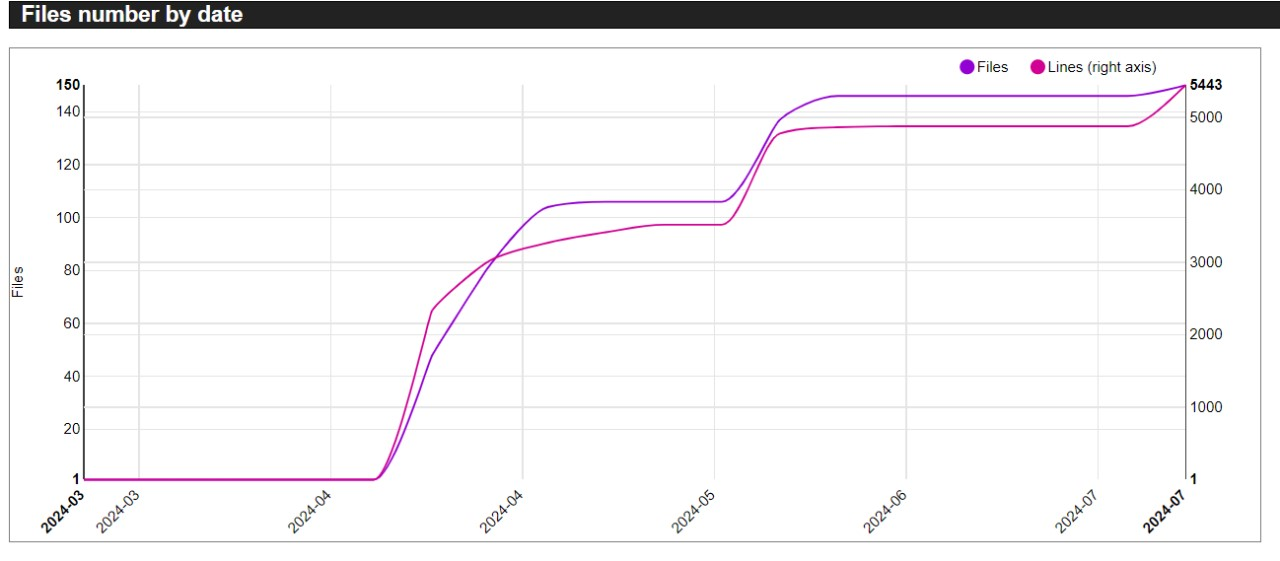
\includegraphics[width=1.0\textwidth]{images/arquivos-por-data-stats-back.jpg}
        \caption{Gráfico com a relação número de arquivos adicionados e linhas de código}
        \label{fig:arquivosPorDataBack}
    \end{figure}


Na figura \ref{fig:tiposdeArquivosBack} são apresentados os dados referentes ao tipo de arquivo presente no projeto \textit{back-end}.

\begin{figure}[ht]
        \centering
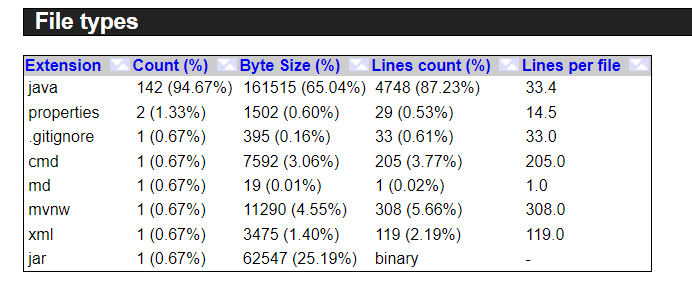
\includegraphics[width=1.0\textwidth]{images/tipos-arquivos-stats-back.png}
        \caption{Tipos de arquivos presentes no repositório do projeto \textit{back-end} do GitHub}
        \label{fig:tiposdeArquivosBack}
    \end{figure}

\newpage

Na figura \ref{fig:infoArquivosBack} são apresentados os dados gerais referente aos arquivos presentes no projeto \textit{back-end}.

    \begin{figure}[ht]
        \centering
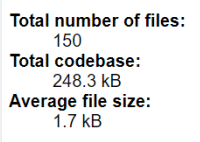
\includegraphics[width=0.5\textwidth]{images/info-arquivos-stats-back.png}
        \caption{Dados de arquivos presentes no repositório do projeto \textit{back-end}}
        \label{fig:infoArquivosBack}
    \end{figure}


Na figura \ref{fig:dadosGeraisFront}, são apresentados os dados gerais à respeito do repositório GitHub referente ao projeto \textit{front-end}.

\begin{figure}[ht]
        \centering
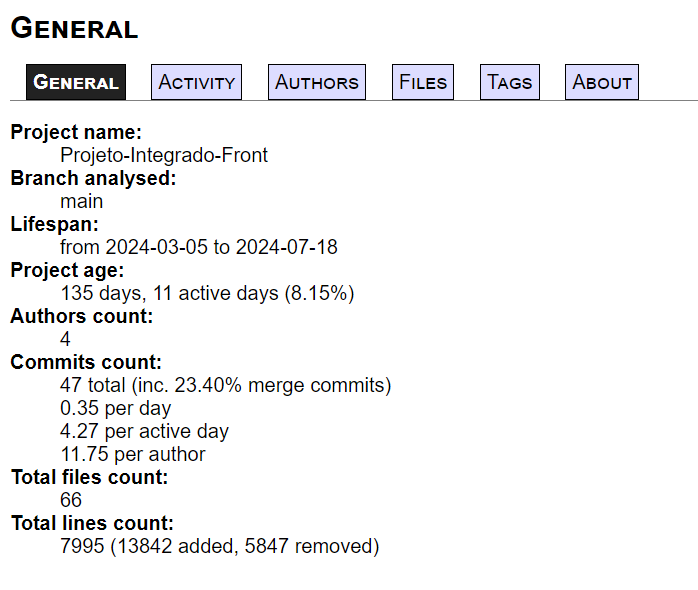
\includegraphics[width=0.65\textwidth]{images/dados-gerais-stats-front.png}
        \caption{Dados Gerais sobre o repositório \textit{front-end} do GitHub}
        \label{fig:dadosGeraisFront}
    \end{figure}

\newpage


Na figura \ref{fig:commitsPorHoraFront} são apresentados os dados referentes à relação entre o dia da semana, e o horário em que foram feitos os commits no repositório do projeto \textit{front-end} do GitHub.

\begin{figure}[ht]
        \centering
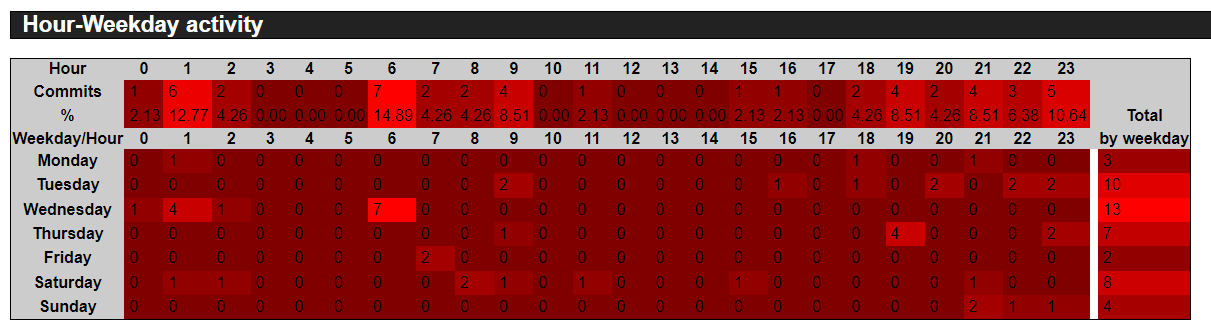
\includegraphics[width=1.0\textwidth]{images/commits-hora-semana-stats-front.png}
        \caption{Dados Gerais sobre o repositório \textit{front-end} do GitHub}
        \label{fig:commitsPorHoraFront}
    \end{figure}

Na figura \ref{fig:commitsPorMesFront} são apresentados os dados referentes ao número de commits em cada mês do ano de 2024 referente ao repositório do projeto \textit{front-end} do GitHub.

\begin{figure}[ht]
        \centering
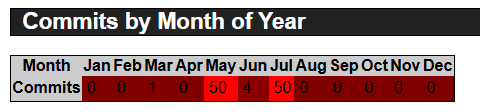
\includegraphics[width=0.75\textwidth]{images/commits-mes-stats-front.png}
        \caption{Número de commits em cada mês do ano de 2024}
        \label{fig:commitsPorMesFront}
    \end{figure}

Na figura \ref{fig:commitsPorAutorFront} são apresentados os dados referentes ao número de commits por autor no repositório do projeto \textit{front-end} do GitHub.  

\begin{figure}[ht]
        \centering
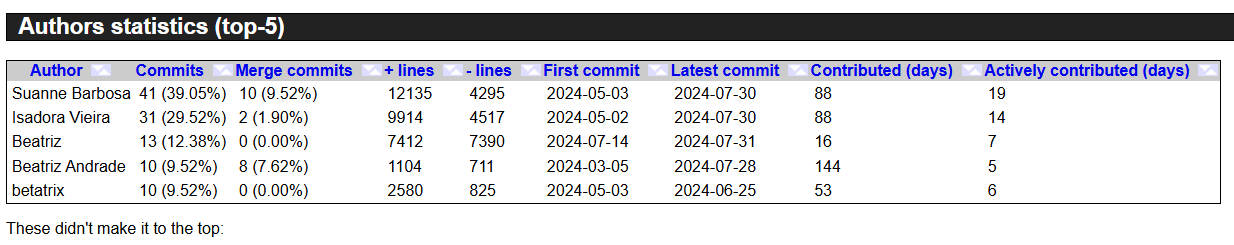
\includegraphics[width=1.0\textwidth]{images/autor-stats-front.png}
        \caption{Número de commits por autor}
        \label{fig:commitsPorAutorFront}
    \end{figure}

\newpage

Na figura \ref{fig:linhasPorAutorFront} é apresentado o gráfico referente ao número de linhas de código adicionadas por autor no repositório do projeto \textit{front-end} do GitHub.  

\begin{figure}[ht]
        \centering
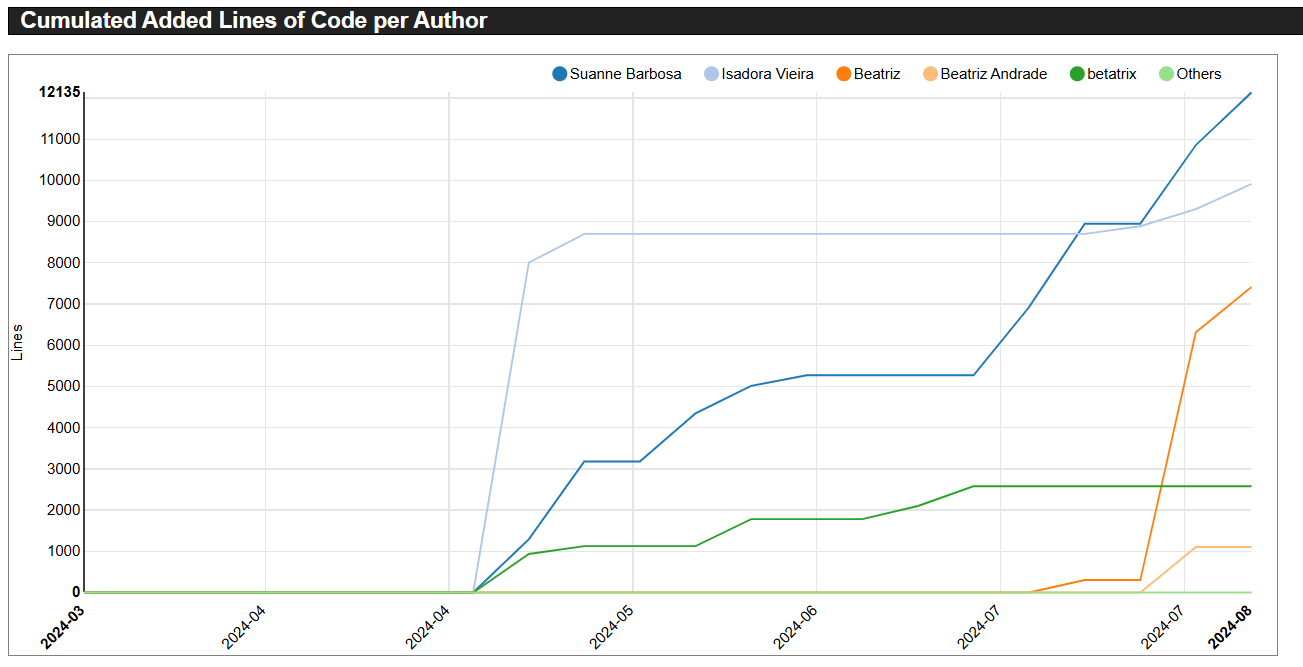
\includegraphics[width=1.0\textwidth]{images/linhas-por-autor-stats-front.png}
        \caption{Número de linhas de código por autor}
        \label{fig:linhasPorAutorFront}
    \end{figure}


Na figura \ref{fig:graficoCommitsPorAutorFront} é apresentado o gráfico referente ao número de commits por autor no repositório do projeto \textit{front-end} do GitHub.  

\begin{figure}[ht]
        \centering
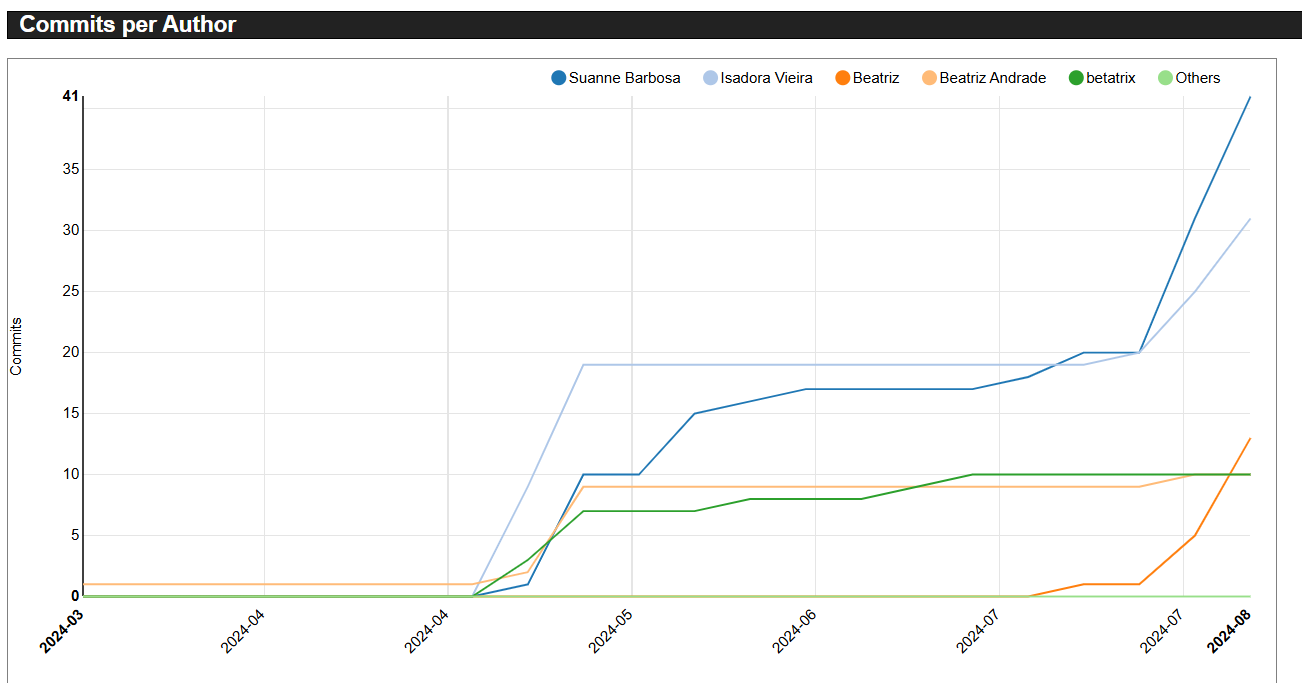
\includegraphics[width=1.0\textwidth]{images/commits-autor-stats-front.png}
        \caption{Gráfico número de commits por autor}
        \label{fig:graficoCommitsPorAutorFront}
    \end{figure}

\newpage

A figura \ref{fig:graficoCommitsPorAutorFront2} é um complemento do gráfico da figura 30, no qual é apresentado o gráfico referente ao número de commits por autor no repositório do projeto \textit{front-end} do GitHub.  

\begin{figure}[ht]
        \centering
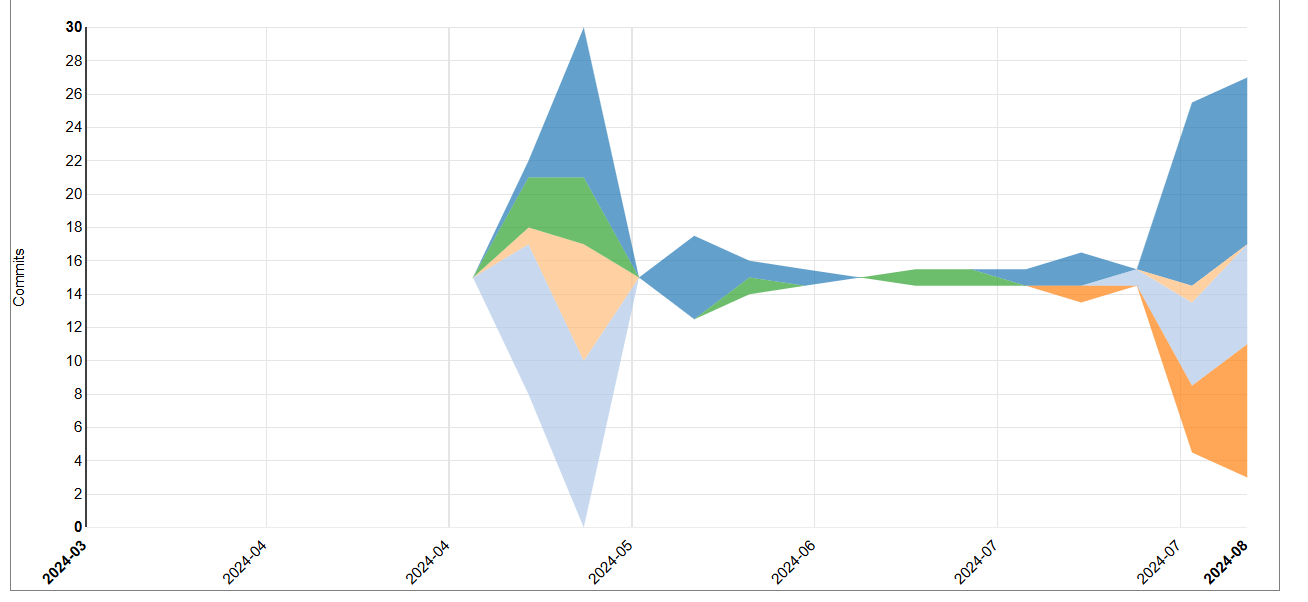
\includegraphics[width=1.0\textwidth]{images/commits-autor2-stats-front.png}
        \caption{Gráfico número de commits por autor}
        \label{fig:graficoCommitsPorAutorFront2}
    \end{figure}


Na figura \ref{fig:rankingAutoresFront} é apresentado o ranking dos autores com o maior número de commits em cada mês do ano de 2024 no repositório do projeto \textit{front-end} do GitHub.  

\begin{figure}[ht]
        \centering
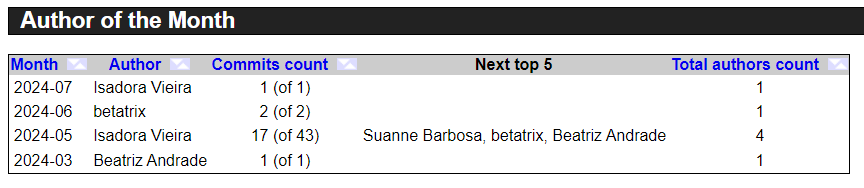
\includegraphics[width=1.0\textwidth]{images/rank-autor-stats-front.png}
        \caption{Tabela autor com o maior número de commits em cada mês do ano de 2024}
        \label{fig:rankingAutoresFront}
    \end{figure}

\newpage

Na figura \ref{fig:numeroLinhasFront} é apresentado o gráfico referente ao número de arquivos adicionados e número de linhas de código no repositório do projeto \textit{front-end} do GitHub no decorrer do primeiro semestre de 2024.

\begin{figure}[ht]
        \centering
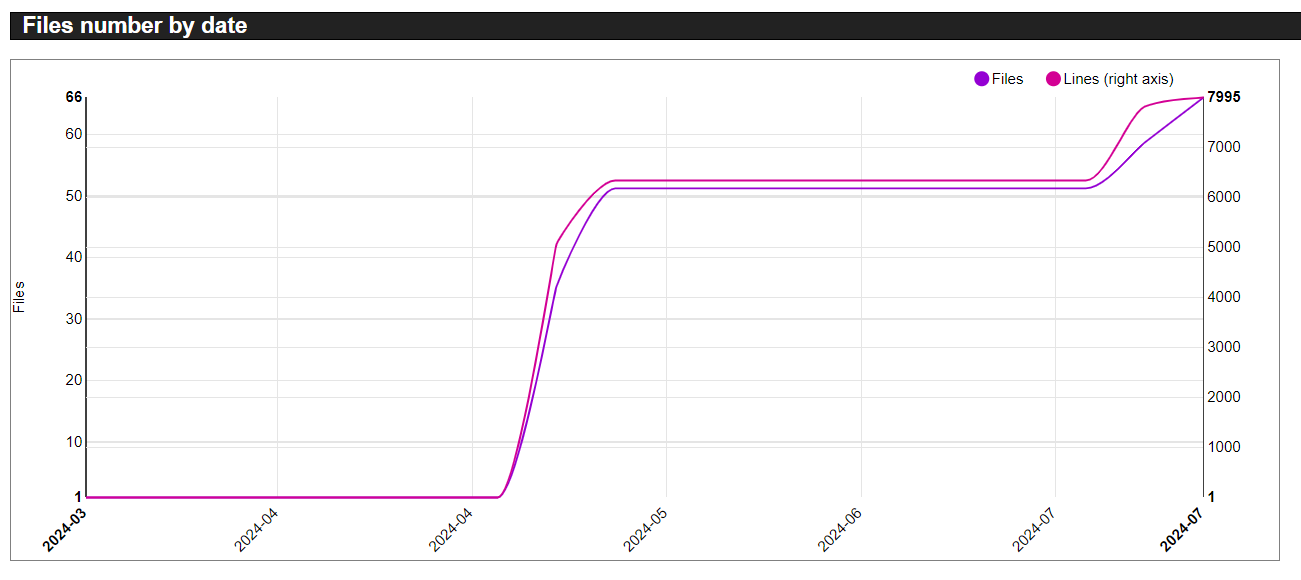
\includegraphics[width=1.0\textwidth]{images/arquivos-por-data-stats-front.png}
        \caption{Gráfico com a relação número de arquivos adicionados e linhas de código}
        \label{fig:numeroLinhasFront}
    \end{figure}

Na figura \ref{fig:tiposdeArquivosFront} são apresentados os dados referentes ao tipo de arquivo presente no projeto \textit{front-end}.

\begin{figure}[ht]
        \centering
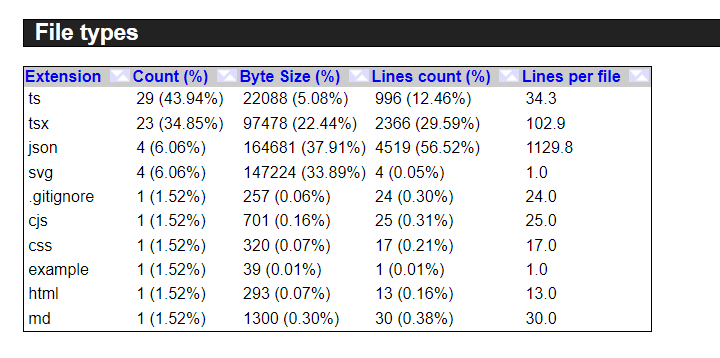
\includegraphics[width=1.0\textwidth]{images/tipos-arquivos-stats-front.png}
        \caption{Tipos de arquivos presentes no repositório do projeto \textit{front-end} do GitHub}
        \label{fig:tiposdeArquivosFront}
    \end{figure}

\newpage


Na figura \ref{fig:infoArquivosFront} são apresentados os dados gerais referente aos arquivos presentes no projeto \textit{front-end}.

    \begin{figure}[ht]
        \centering
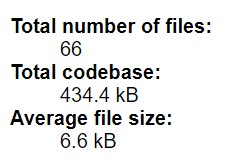
\includegraphics[width=0.5\textwidth]{images/info-arquivos-stats-front.jpg}
        \caption{Dados de arquivos presentes no repositório do projeto \textit{front-end}}
        \label{fig:infoArquivosFront}
    \end{figure}


Com esses dados estatísticos à respeito dos repositórios do projeto Vocco, é possível obter uma visão ampla da evolução desenvolvimento e como a participação de cada integrante do grupo é essencial, auxiliando na construção do sistema como um todo.